\hypertarget{introduction}{%
\section{Introduction}\label{introduction2}}

The motivation of this thesis was twofold: firstly, to produce three-dimensional epithelia with controlled pressure, and secondly, to study the material response of the tissue to different regimes of tension. To achieve the first objective, we have developed a monolayer inflator (MOLI) device that allows us to create epithelial domes where cells can be stretched to more than $100\%$ of areal strain.

Epithelial tissue plays a crucial role in various physiological functions, and must therefore undergo deformation over a wide range of timescales and magnitudes. Similarly, pressure levels also vary widely in different contexts \cite{torres-sanchez2021, choudhury2022a}. For instance, the luminal pressure in blastocysts doubles over the course of its development, resulting in changes in cortical tension and strain \cite{chan2019}. The MDCK dome system provides a suitable platform to investigate the interplay between cell strain, tension, and pressure. Previous studies by Latorre et al. have observed a wide range of pressure throughout the evolution of the dome, and cells have exhibited a range of deformation, including active-superelastic behavior \cite{latorre2018}. However, the control in this system is limited to the footprint of the domes. In this chapter, we aim to utilize the MOLI system to subject tissues to a range of strain and tension regimes.

\hypertarget{measurement-of-dome-mechanics}{%
	\section{Measurement of dome
		mechanics}\label{measurement-of-dome-mechanics}}

\begin{figure}
	\begin{minipage}[c]{0.7\textwidth}
		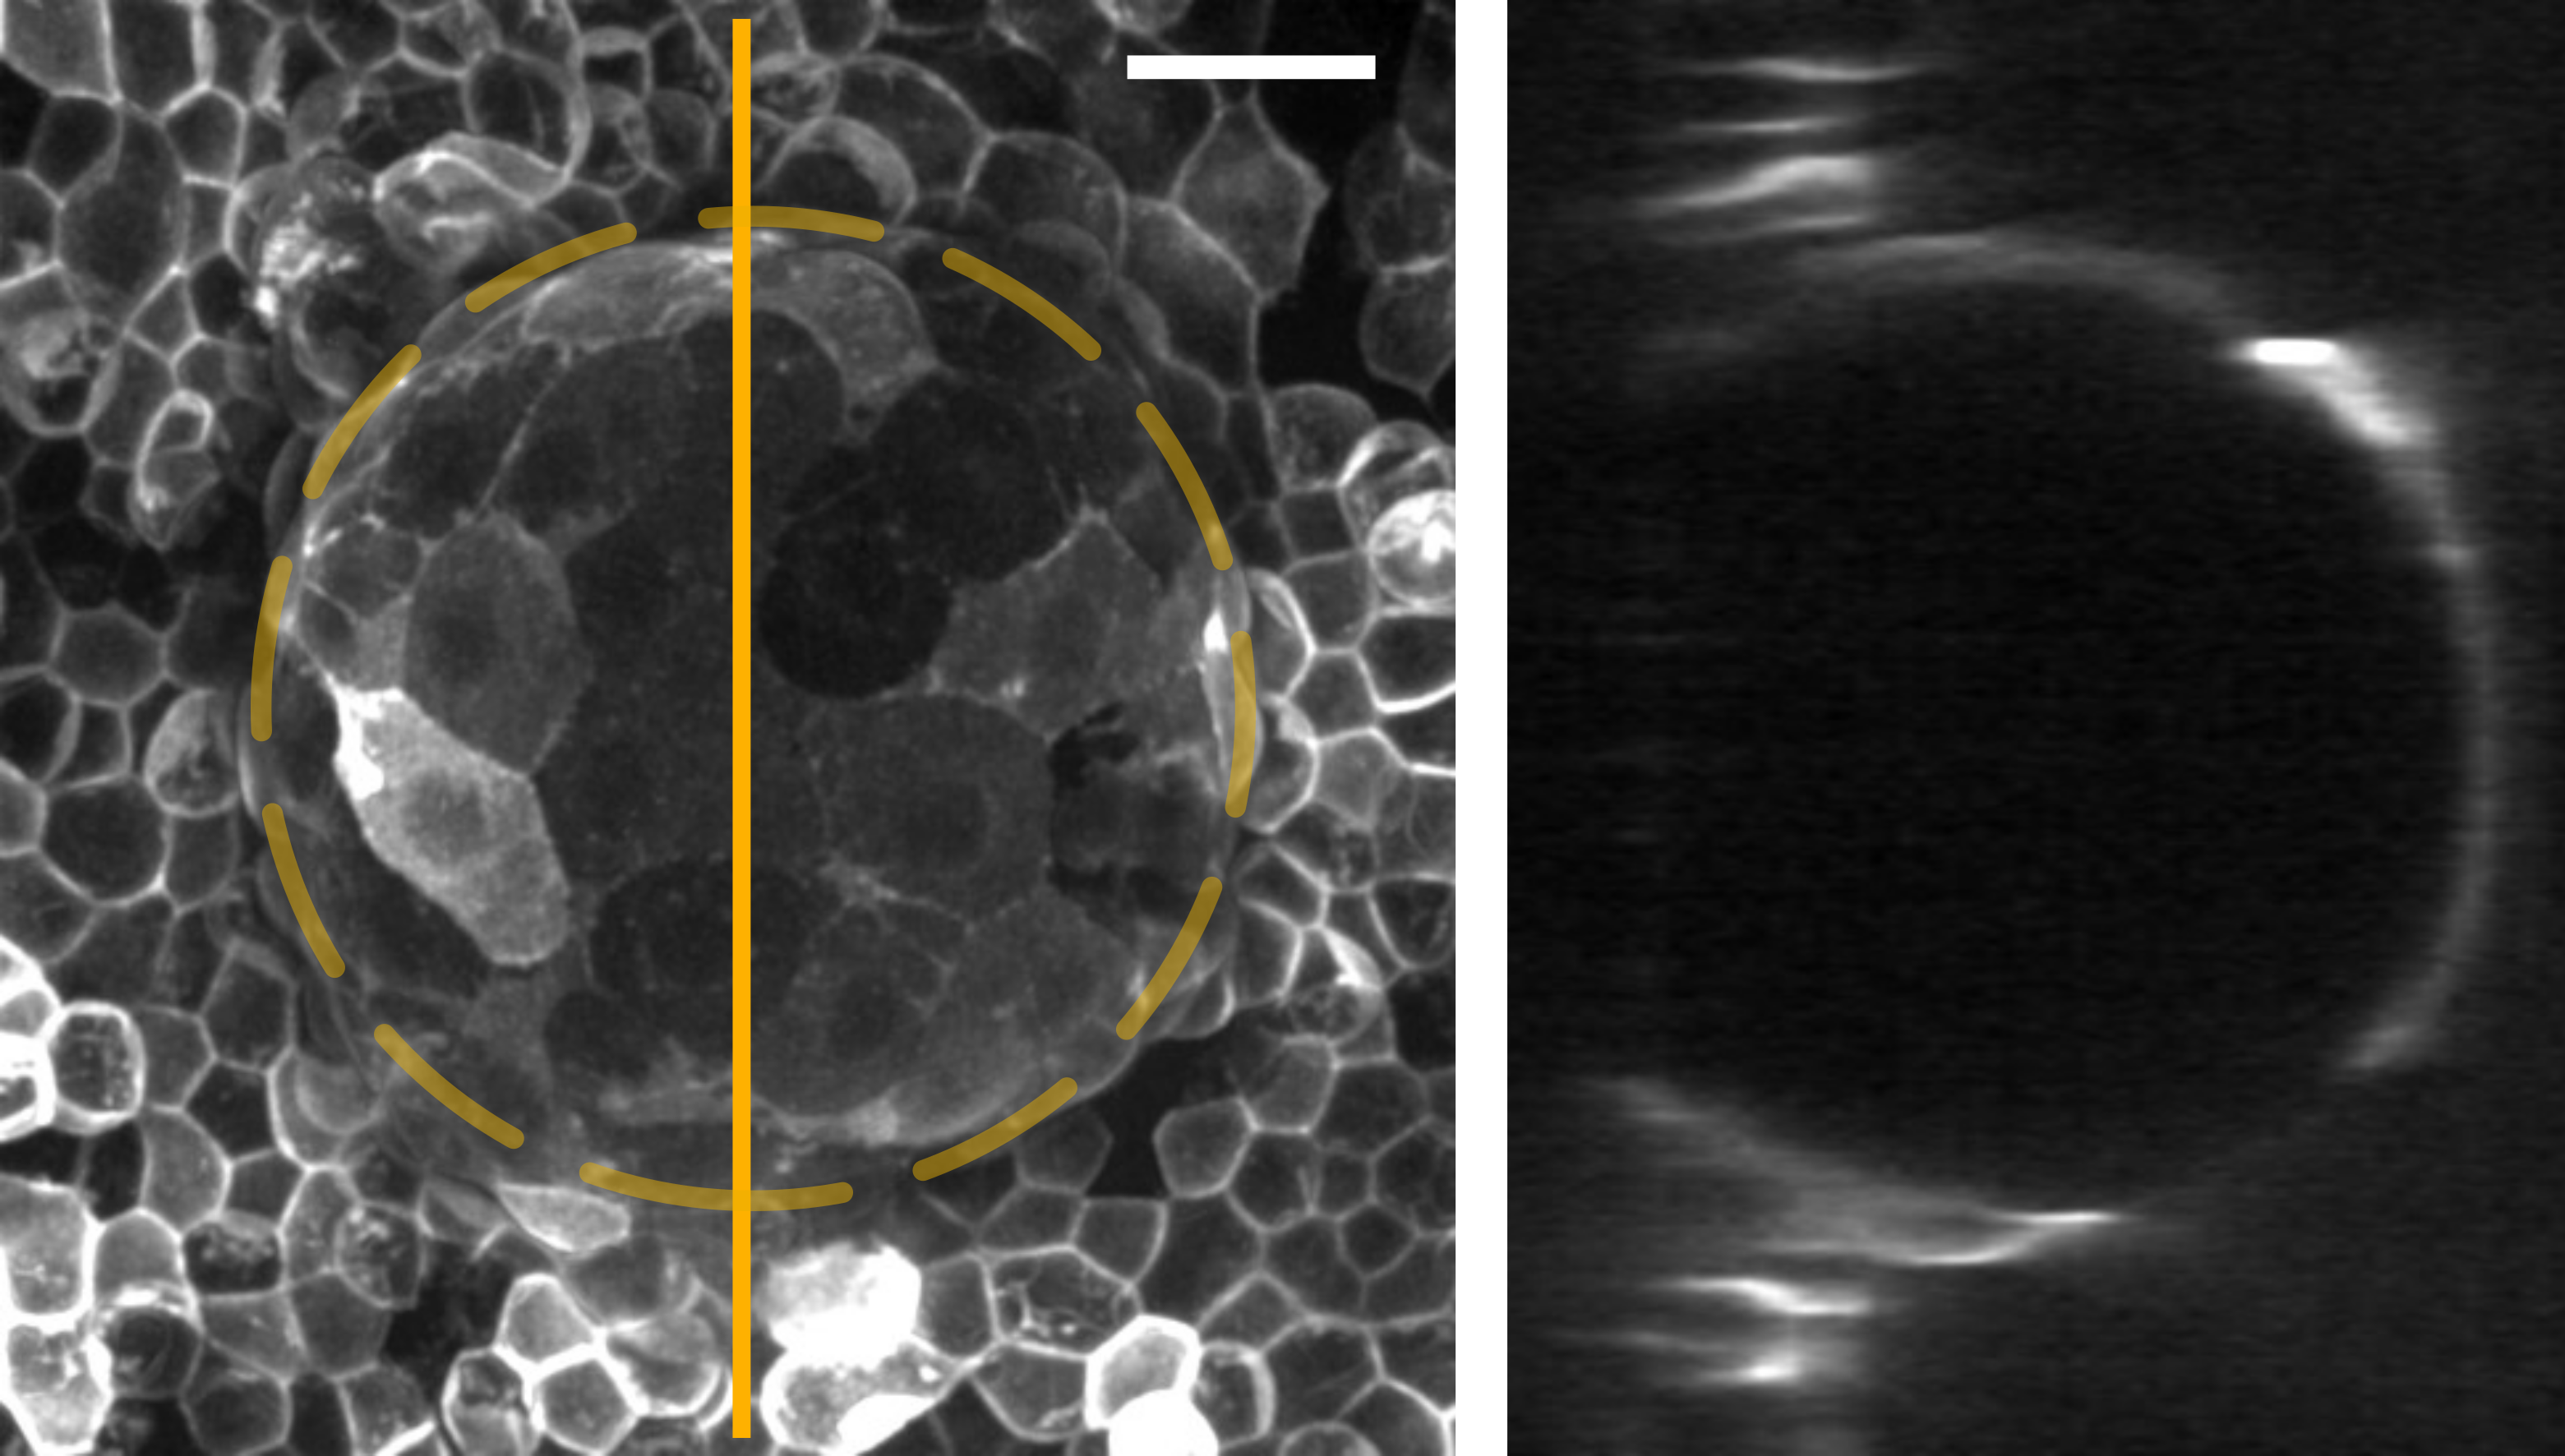
\includegraphics[width=\textwidth]{chap7_realdome.png}
	\end{minipage}\hfill
	\begin{minipage}[c]{0.27\textwidth}
		\caption{\\ \textbf{Spherical cap}:\\Here is an example of an epithelial dome at 200 Pa, which has increased its surface area four times the original footprint. One can clearly appreciate the beautiful spherical shape of the dome in the cross-section. Scale bar is $20 \mu m$.
		} \label{fig_7_1}
	\end{minipage}
\end{figure}

To measure the kinematics of the domes, we analyzed the midsection of the domes, assuming symmetry of spherical caps (see fig \ref{fig_7_1}). We measured the height ($h$) and base radius ($a$). This allowed us to calculate the radius of curvature ($R$) using trigonometry as 
$$ R = \frac{h^2 + a^2}{2h}.$$ 
The measurement of pressure ($\Delta P$) allowed us to compute the tension ($\sigma$), given by Laplace's law 
$$\sigma = \frac{\Delta PR }{2} .$$
For the dome strain, we used the areal strain measure, which is computed based on the surface area. We compared the dome surface area ($A$) to the area of the footprint ($A_{0}$).
$$ \epsilon = \frac{A - A_{0}}{A_{0}} = \frac{\pi(h^2 + a^2) - \pi a^2}{\pi a^2} = \frac{h^2}{a^2} .$$
Using the line scan method of imaging domes for fast time-lapse, we obtained a large number of frames for the analysis of the height and radius of curvature. Thus, we used kymographs of the top section of the dome. Kymographs are images with a cross-section of the dome top with respect to time. Using image processing MATLAB code, we obtained the location of the maximum intensity value for a particular time in the graph to obtain the time evolution of the height of the dome. The same method was used for the base radius as well. The kymograph of the base radius allowed us to keep track of delamination, as it could change the value of strain.

\hypertarget{epithelial-domes-at-constant-pressure}{%
	\section{Epithelial domes at constant
		pressure}\label{epithelial-domes-at-constant-pressure}}


\begin{figure}
	\centering
	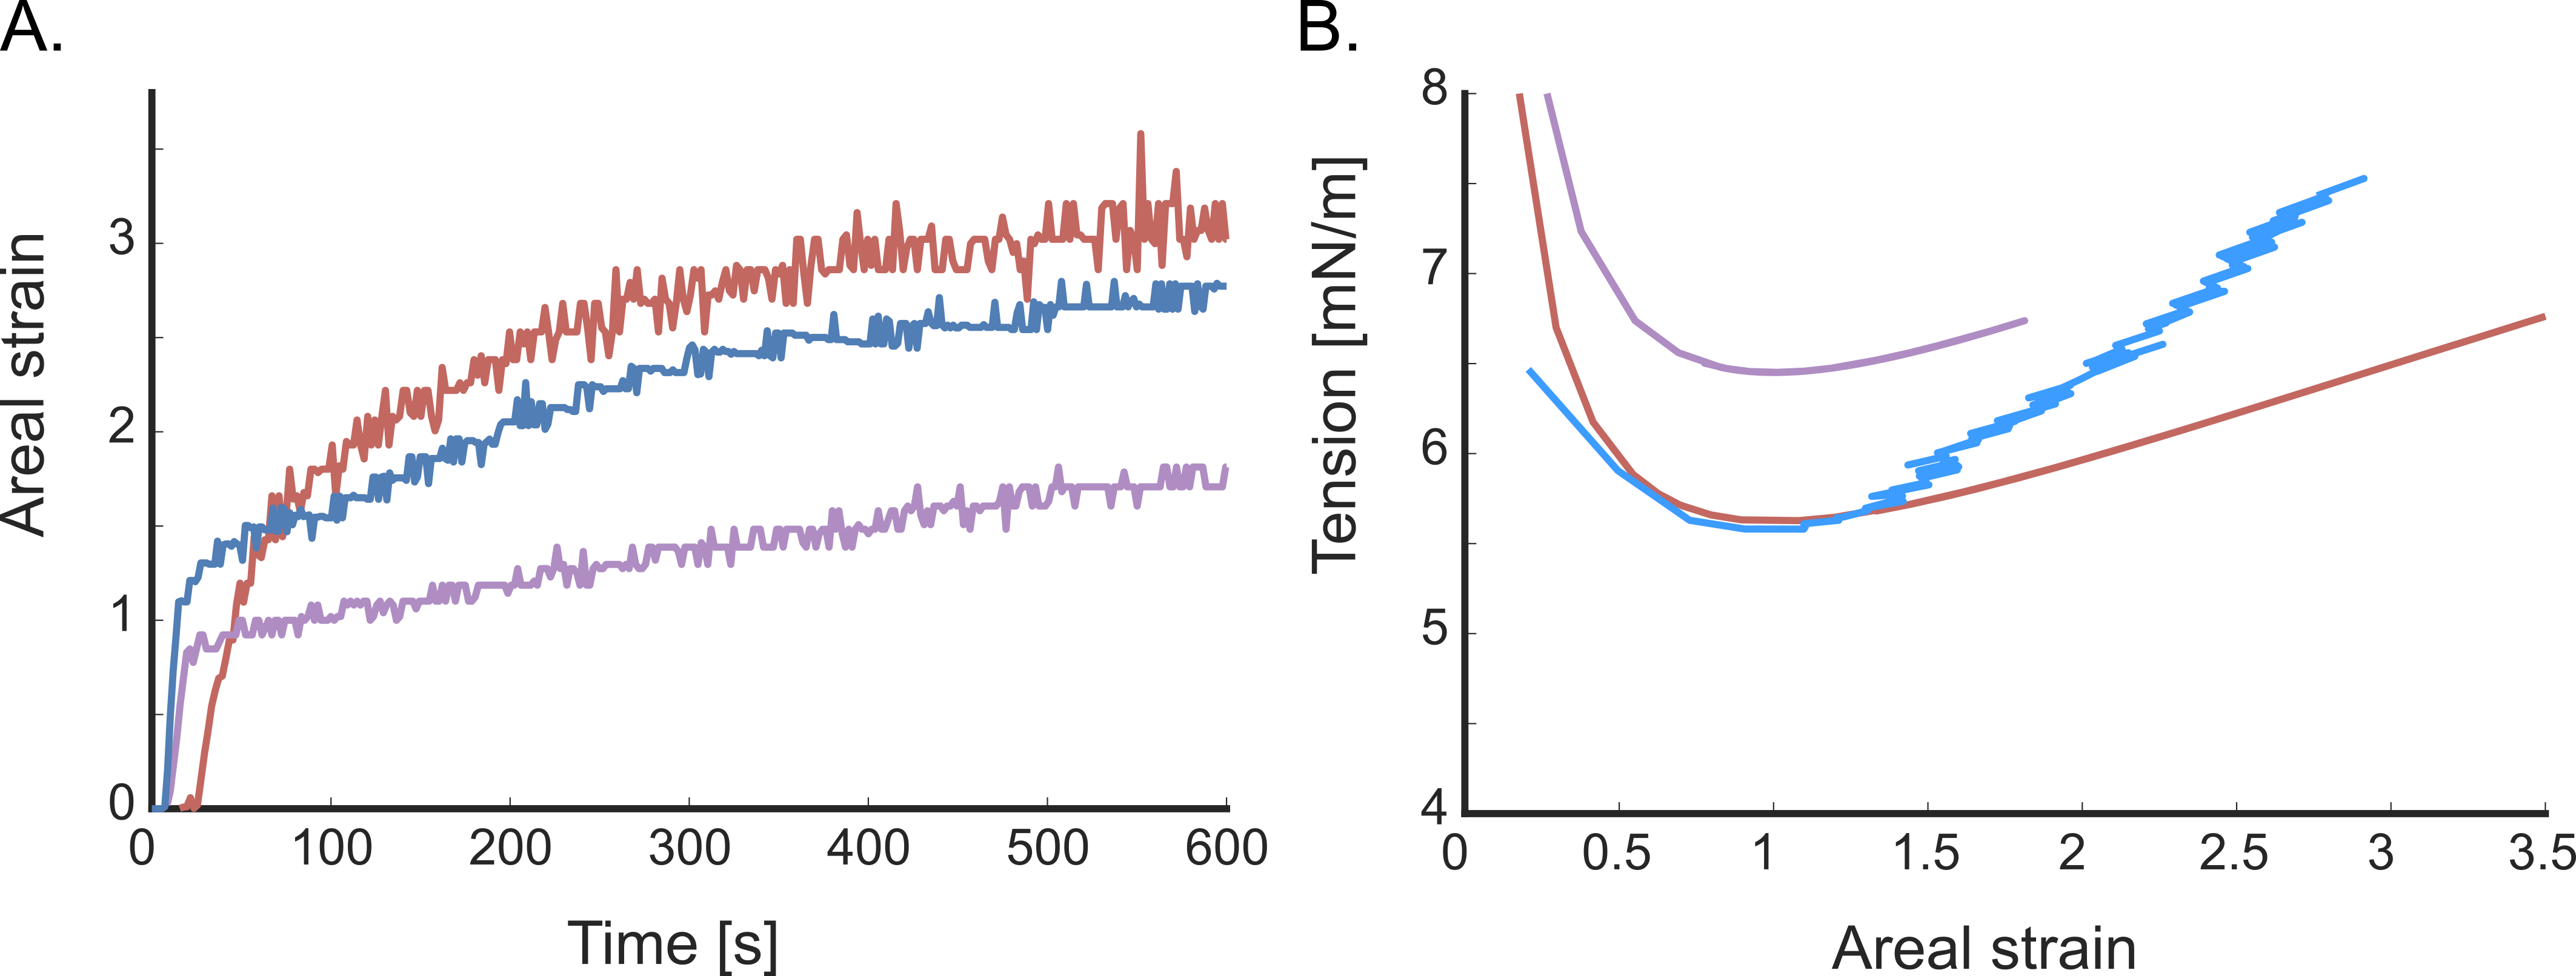
\includegraphics[width=\textwidth]{chap7_constpressure.png}
	\caption{\label{fig_7_3} \textbf{Epithelial domes at constant pressure}:Dynamic response of the representative domes at a constant pressure of 200 Pa: (A) Areal strain increases and reaches a steady state at around 5 minutes, and we can clearly see variability in the maximum strains. (B) The same domes produce a peculiar "NIKE swish" shaped tension and strain curve.
	}
\end{figure}

Initially, our focus was to investigate the behavior of domes under constant pressure. We conducted experiments inflating domes at varying pressures, but observed that hardly any of the domes formed at pressures lower than $50-100 Pa$. After optimizing for different pressures, we settled on using $200 Pa$ which allowed domes to form without delaminating out of pattern.

Our results indicate that the areal strain of the dome increases during the first $3-5$ minutes of pressure application, and then reaches a plateau in strain until $5-10$ minutes (see fig \ref{fig_7_3} A). Despite large dome-to-dome variability, with strains ranging from $50\%$ to $300\%$, the stabilization in strain suggests that a steady state has been achieved by the tissue.

Further examination of the tension-strain relationship of these domes revealed a distinctive curve, resembling the swish symbol of "Nike" (see fig \ref{fig_7_3} B). The tension is extremely high for low strains, and then decreases to a minimum around an areal strain of one, where the dome forms a perfect hemisphere. The tension increases again, but the slope is relatively gentle as compared to the steep decline observed at low strains.

This kind of material response would be unusual for typical materials undergoing biaxial stretching. However, in our case, the underlying cause of this curve can be attributed to the geometric constraint imposed by the dome system and force balance (Laplace's law). Since the tension in the dome is a function of its radius of curvature, the radius of curvature starts out very high, producing higher tension that then reduces to a minimum with a hemispherical shape before increasing again (see fig \ref{fig_7_4}). The radius of curvature, areal strain, and tension are inherently interconnected, such that at a constant pressure, we can write the expression of the curve.

$$ R = \frac{h^2 + a^2}{2h}, \ \ \ \ \text{and} \ \ \ \ \epsilon = \frac{h^2}{a^2}$$
By substituting ($\epsilon$) in ($R$),
$$ R = \frac{h^2/a^2 + 1}{2h/a^2} = a\frac{\epsilon + 1}{\sqrt{\epsilon}}$$
By substituting ($R$) in Laplace's law, we get the relation
$$ \frac{\sigma}{a} = \frac{\Delta P}{4} \left( \frac{\epsilon + 1}{\sqrt{\epsilon}} \right)$$

Normalizing the tension with the base radius results in all domes collapsing onto one curve corresponding to a specific pressure. We call this curve the "isobaric" curve.

In terms of physics, we understand that when the step pressure is applied, the dome suddenly inflates and has to undergo non-steady state out-of-equilibrium stresses. It is clear that this curve does not represent the quasi-static constitutive relation of the epithelial tissue.

\begin{figure}
	\centering
	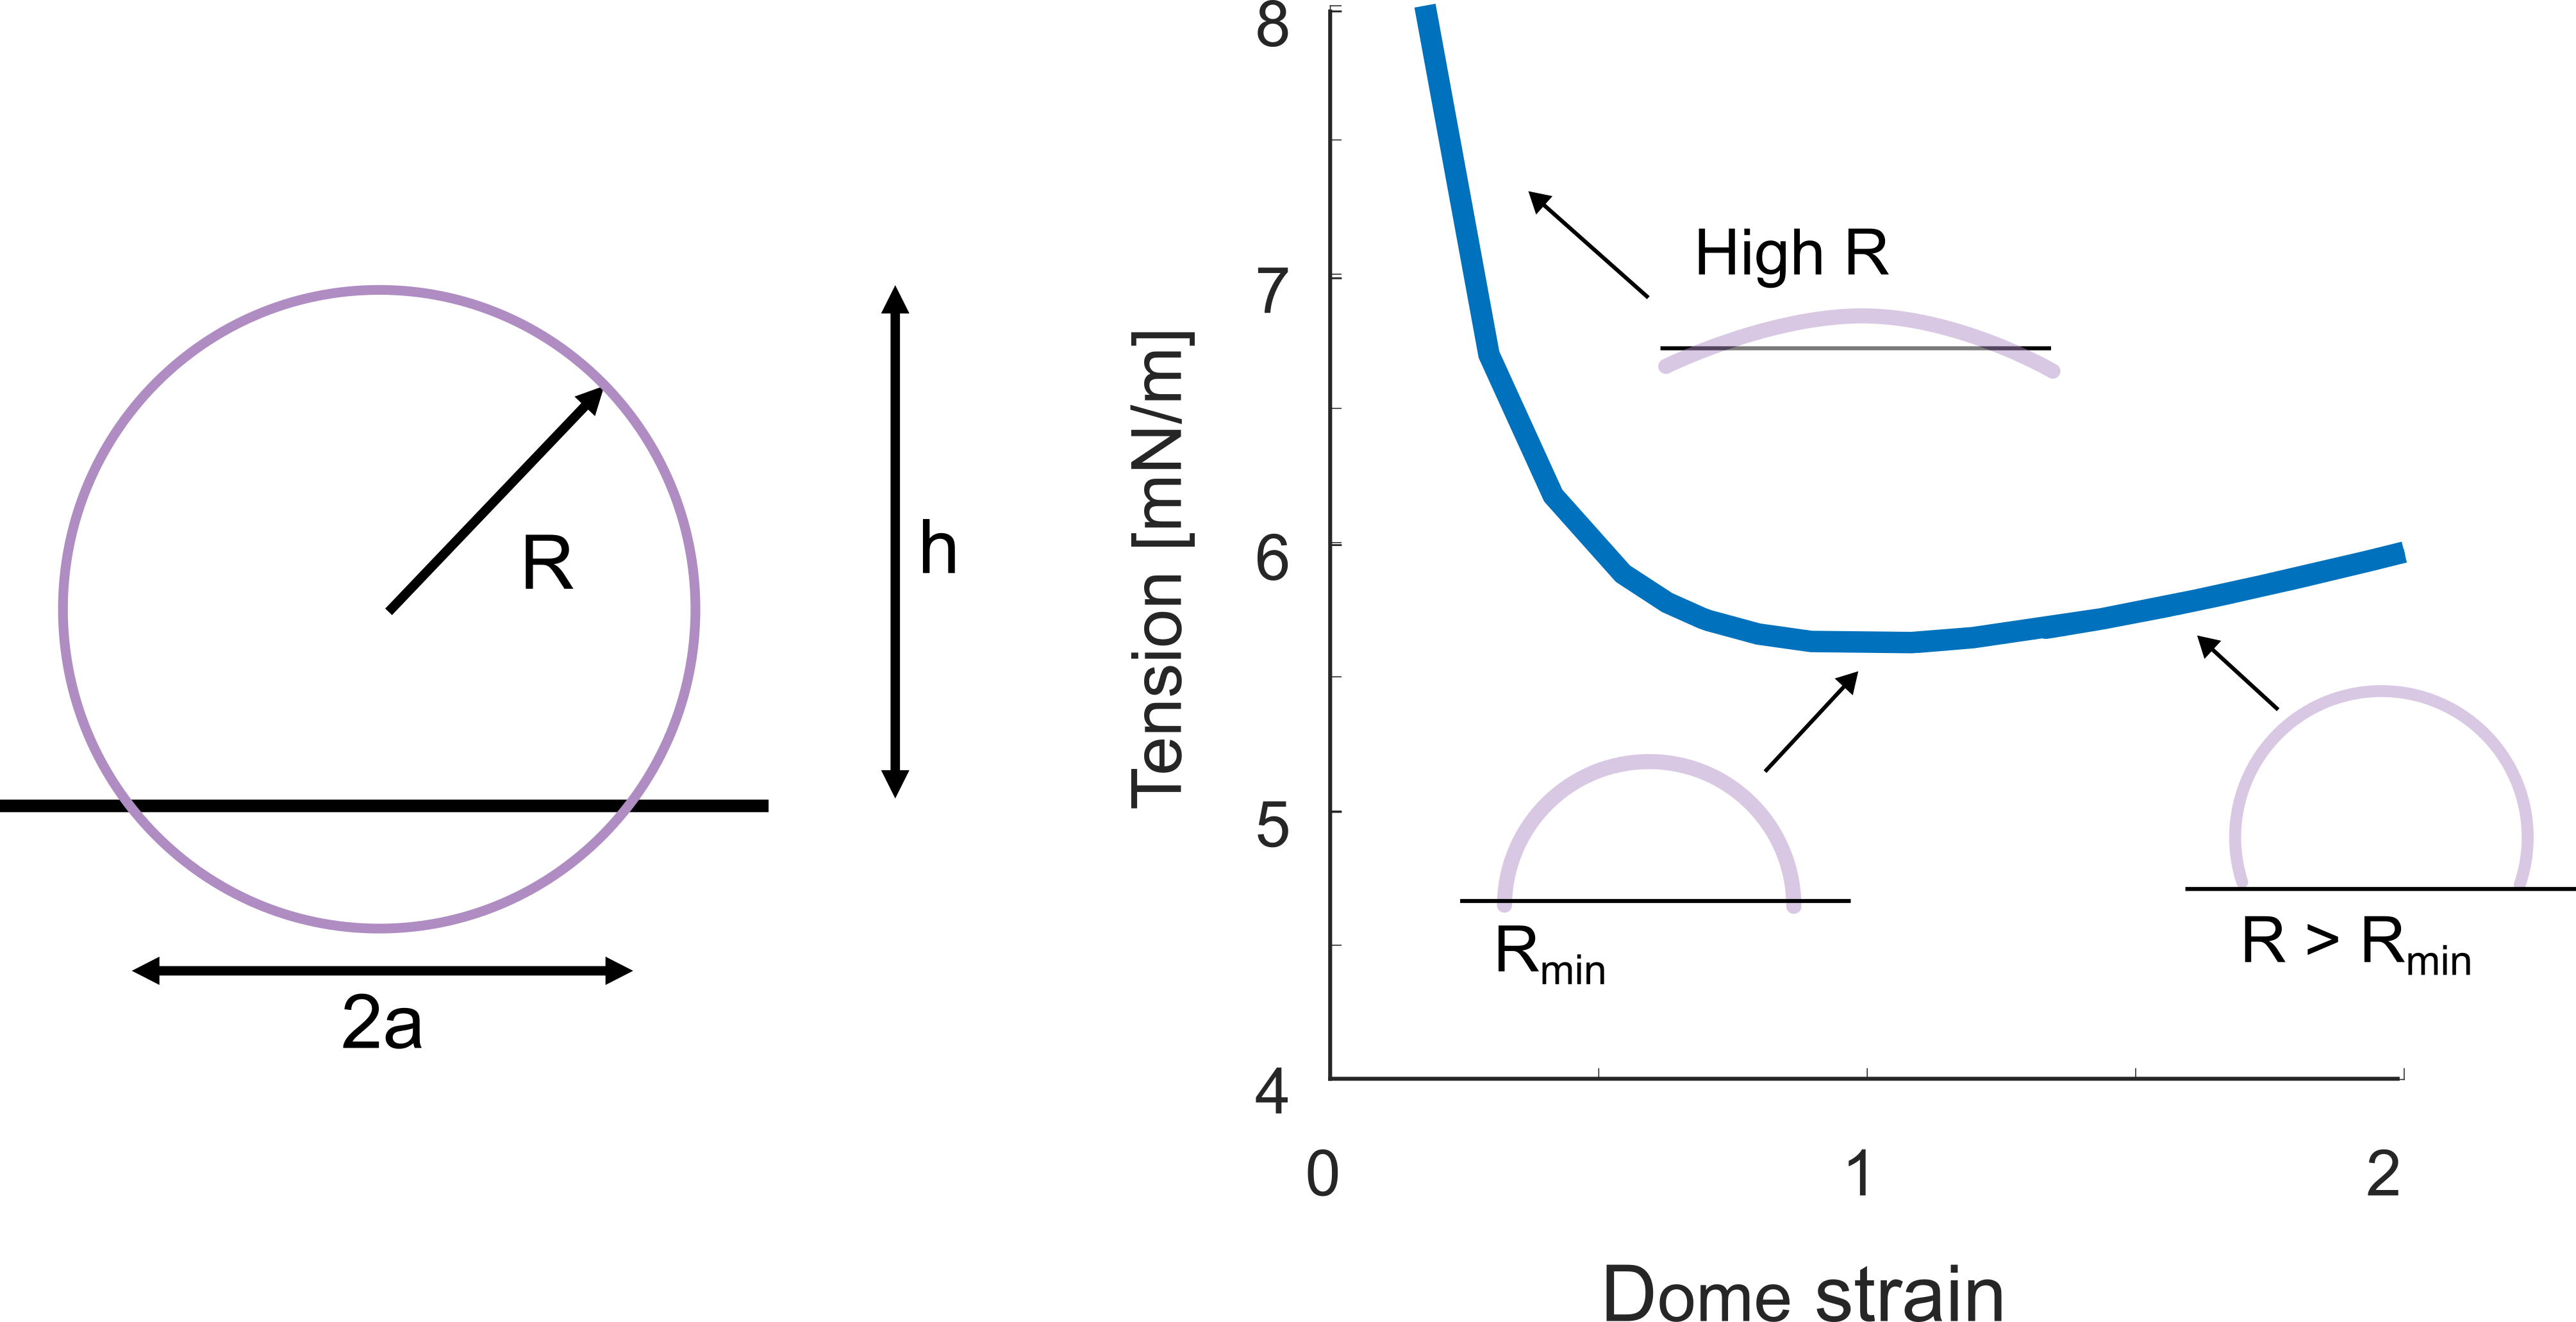
\includegraphics[width=0.8\textwidth]{chap7_radius.png}
	\caption{\label{fig_7_4} \textbf{Illustrative explanation for isobaric curve}: Tension and strain are related to each other through the geometric constraint of a spherical cap. Here, the base radius (a) is constant, so the radius of curvature is almost infinite for domes with very small strains (<0.05). As the strain increases, the radius of curvature decreases to a minimum corresponding to the base radius. Then it continues to increase again.	
	}
\end{figure}



\hypertarget{constitutive-relation-of-epithelia}{%
	\section{Constitutive relation of
		epithelia}\label{constitutive-relation-of-epithelia}}

To obtain the actual constitutive relation, it is preferable to apply strain or tension to a material in a quasi-static manner. However, in our experimental system, only pressure can be controlled. Therefore, we utilized pressure control to achieve steady state tension across a range of strains. Slowly increasing pressure was not practical for domes, as they do not delaminate at low pressures. If delamination did occur, the domes would rapidly inflate and achieve the steady state at higher strains. Consequently, we would not be able to access steady state tensions at lower strains. To address this limitation, we designed experiments for capturing the steady state of the domes by deflating them.

We applied a pressure of 200 Pa for 5 minutes until the dome reached a steady state. Then, we reduced the pressure in steps of 20 Pa and waited for the dome to reach a steady state at each step (see fig \ref{fig_7_5} A). We repeated this process until the dome was completely deflated. In this way, the tension-strain curves captured as the dome passed through different isobarics.

Ultimately, we obtained a constitutive relation that exhibits a initial increase in tension with  strain for lower strains. However, for larger strains, the tension seems to plateau consistently with earlier studies of MDCK domes (see fig \ref{fig_7_5} B). It is worth noting that the variability in dome-to-dome tension is significant, and the tensions recorded around $4.5 mN/m$ are of the same order of magnitude as in previous studies \cite{latorre2018, marin-llaurado2022}.

\begin{figure}
	\centering
	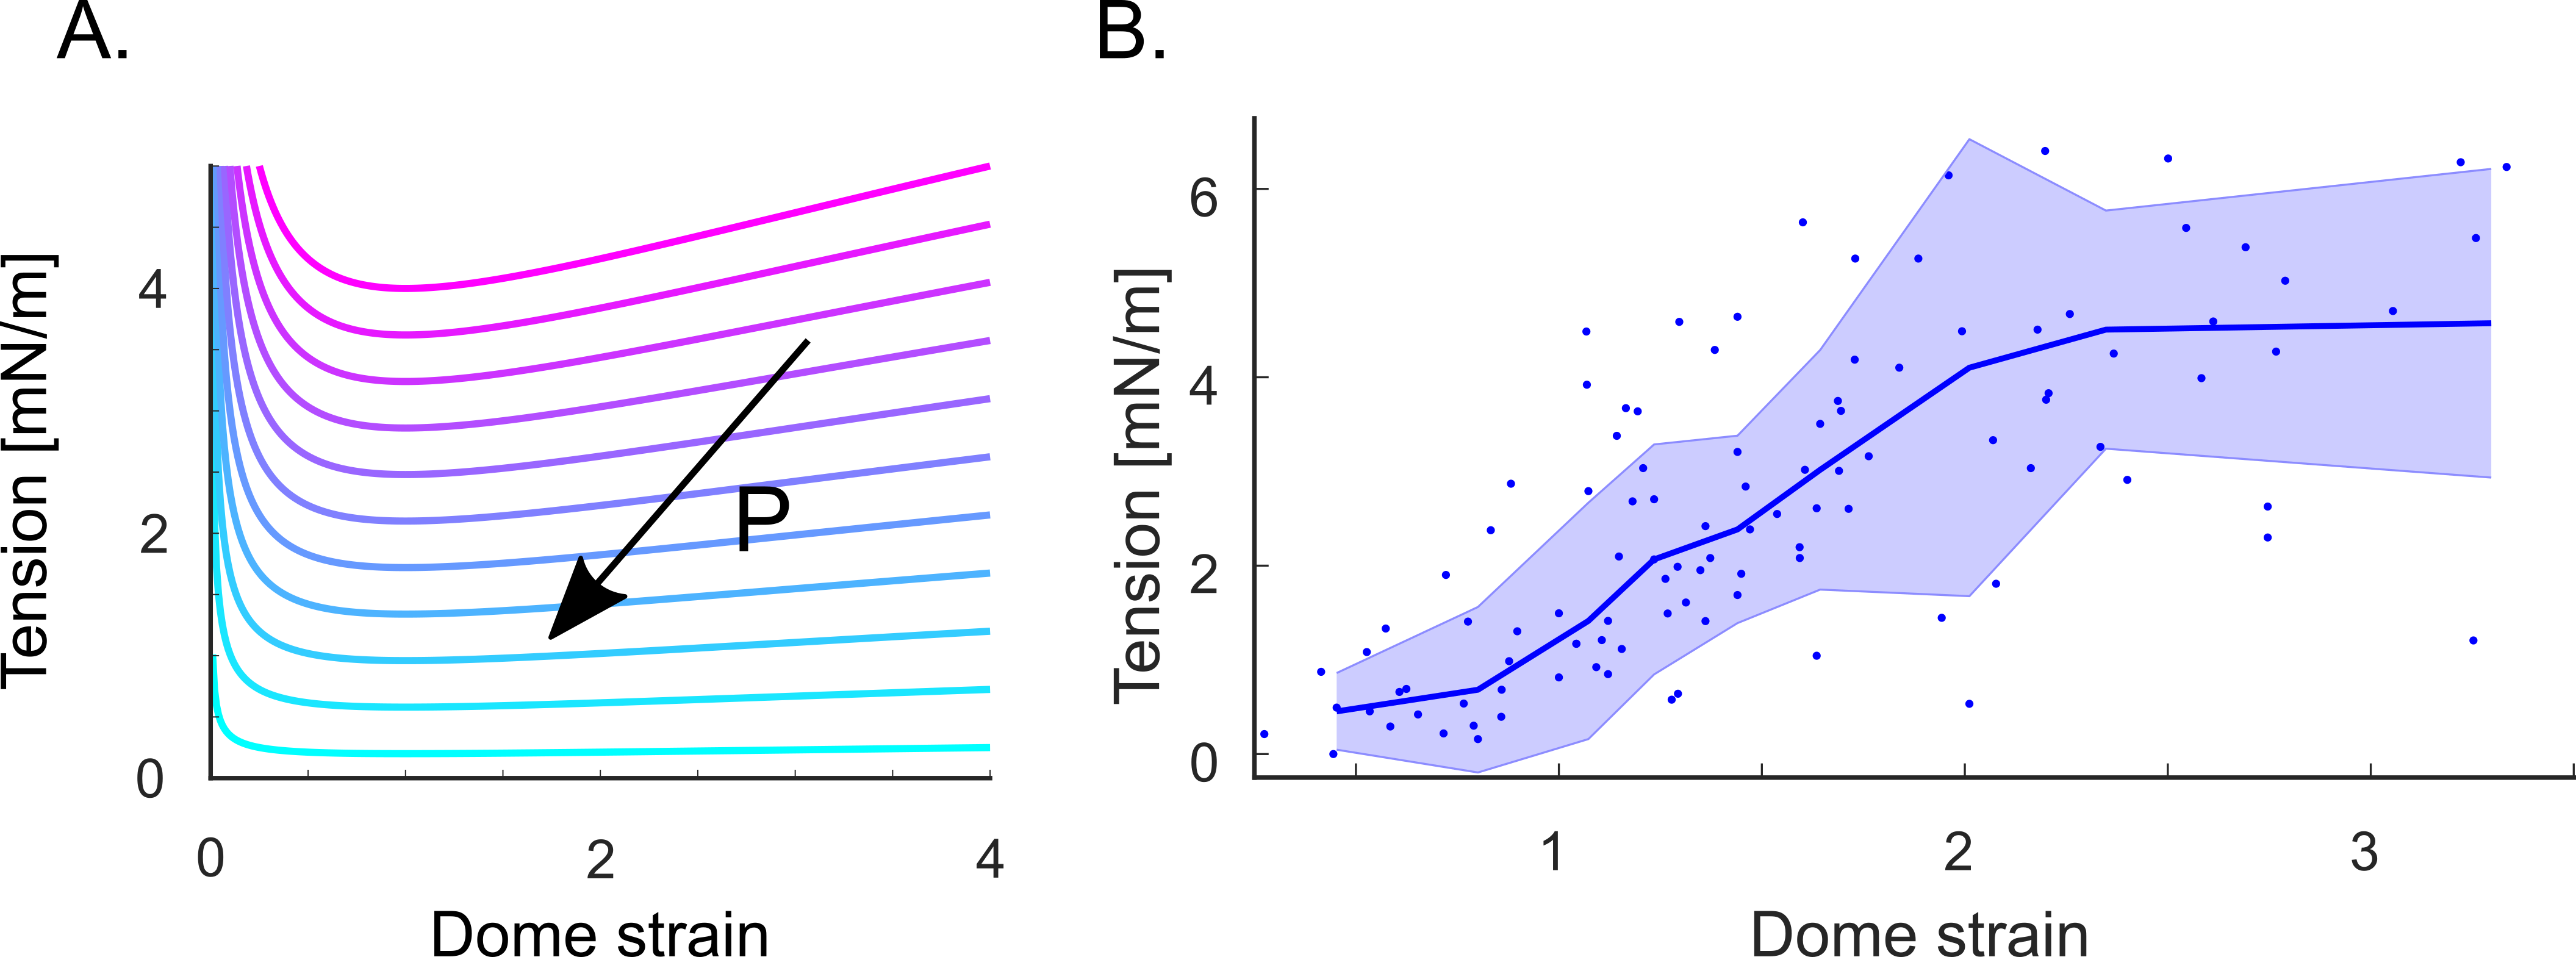
\includegraphics[width=\textwidth]{chap7_constitutivelaw.png}
	\caption{\label{fig_7_5} \textbf{Constitutive Relation of Epithelia}: (A) We will set up experiments to probe the steady state at different pressures. We will start from the highest pressure, move along the isobaric line and achieve a steady state, and then move down to the next isobaric line, and so on.	(B) The constitutive relation between dome strain and tissue tension was experimentally obtained (n=12). The line and shaded area represent the median and standard deviation, respectively, by binning 13 points in each bin.
	}
\end{figure}


\hypertarget{dynamics-of-the-epithelia-domes}{%
	\section{Dynamics of the epithelia
		domes}\label{dynamics-of-the-epithelia-domes}}
	

To investigate the dynamic material response of the domes, we conducted cyclic stretching experiments by subjecting them to a triangular wave of pressure with a magnitude of 200 Pa at three different timescales (see fig \ref{fig_7_6}). Based on the literature on cell remodeling and experimental conditions, we chose cycles of $20 s$, $266 s$, and $2000 s$ \cite{wyatt2016, khalilgharibi2019, casares2015}.

\begin{center}
	\begin{table}[h!]
		\begin{tabular}{c c c c}
			& Fast & Moderate & Slow \\ 
			Time period (s) & 20   & 266      & 2000 \\ 
			Rates (Pa/s)    & 20   & 1.5      & 0.2  \\ 
		\end{tabular}
	\end{table}
\end{center}

\begin{figure}[h!]
	\centering
	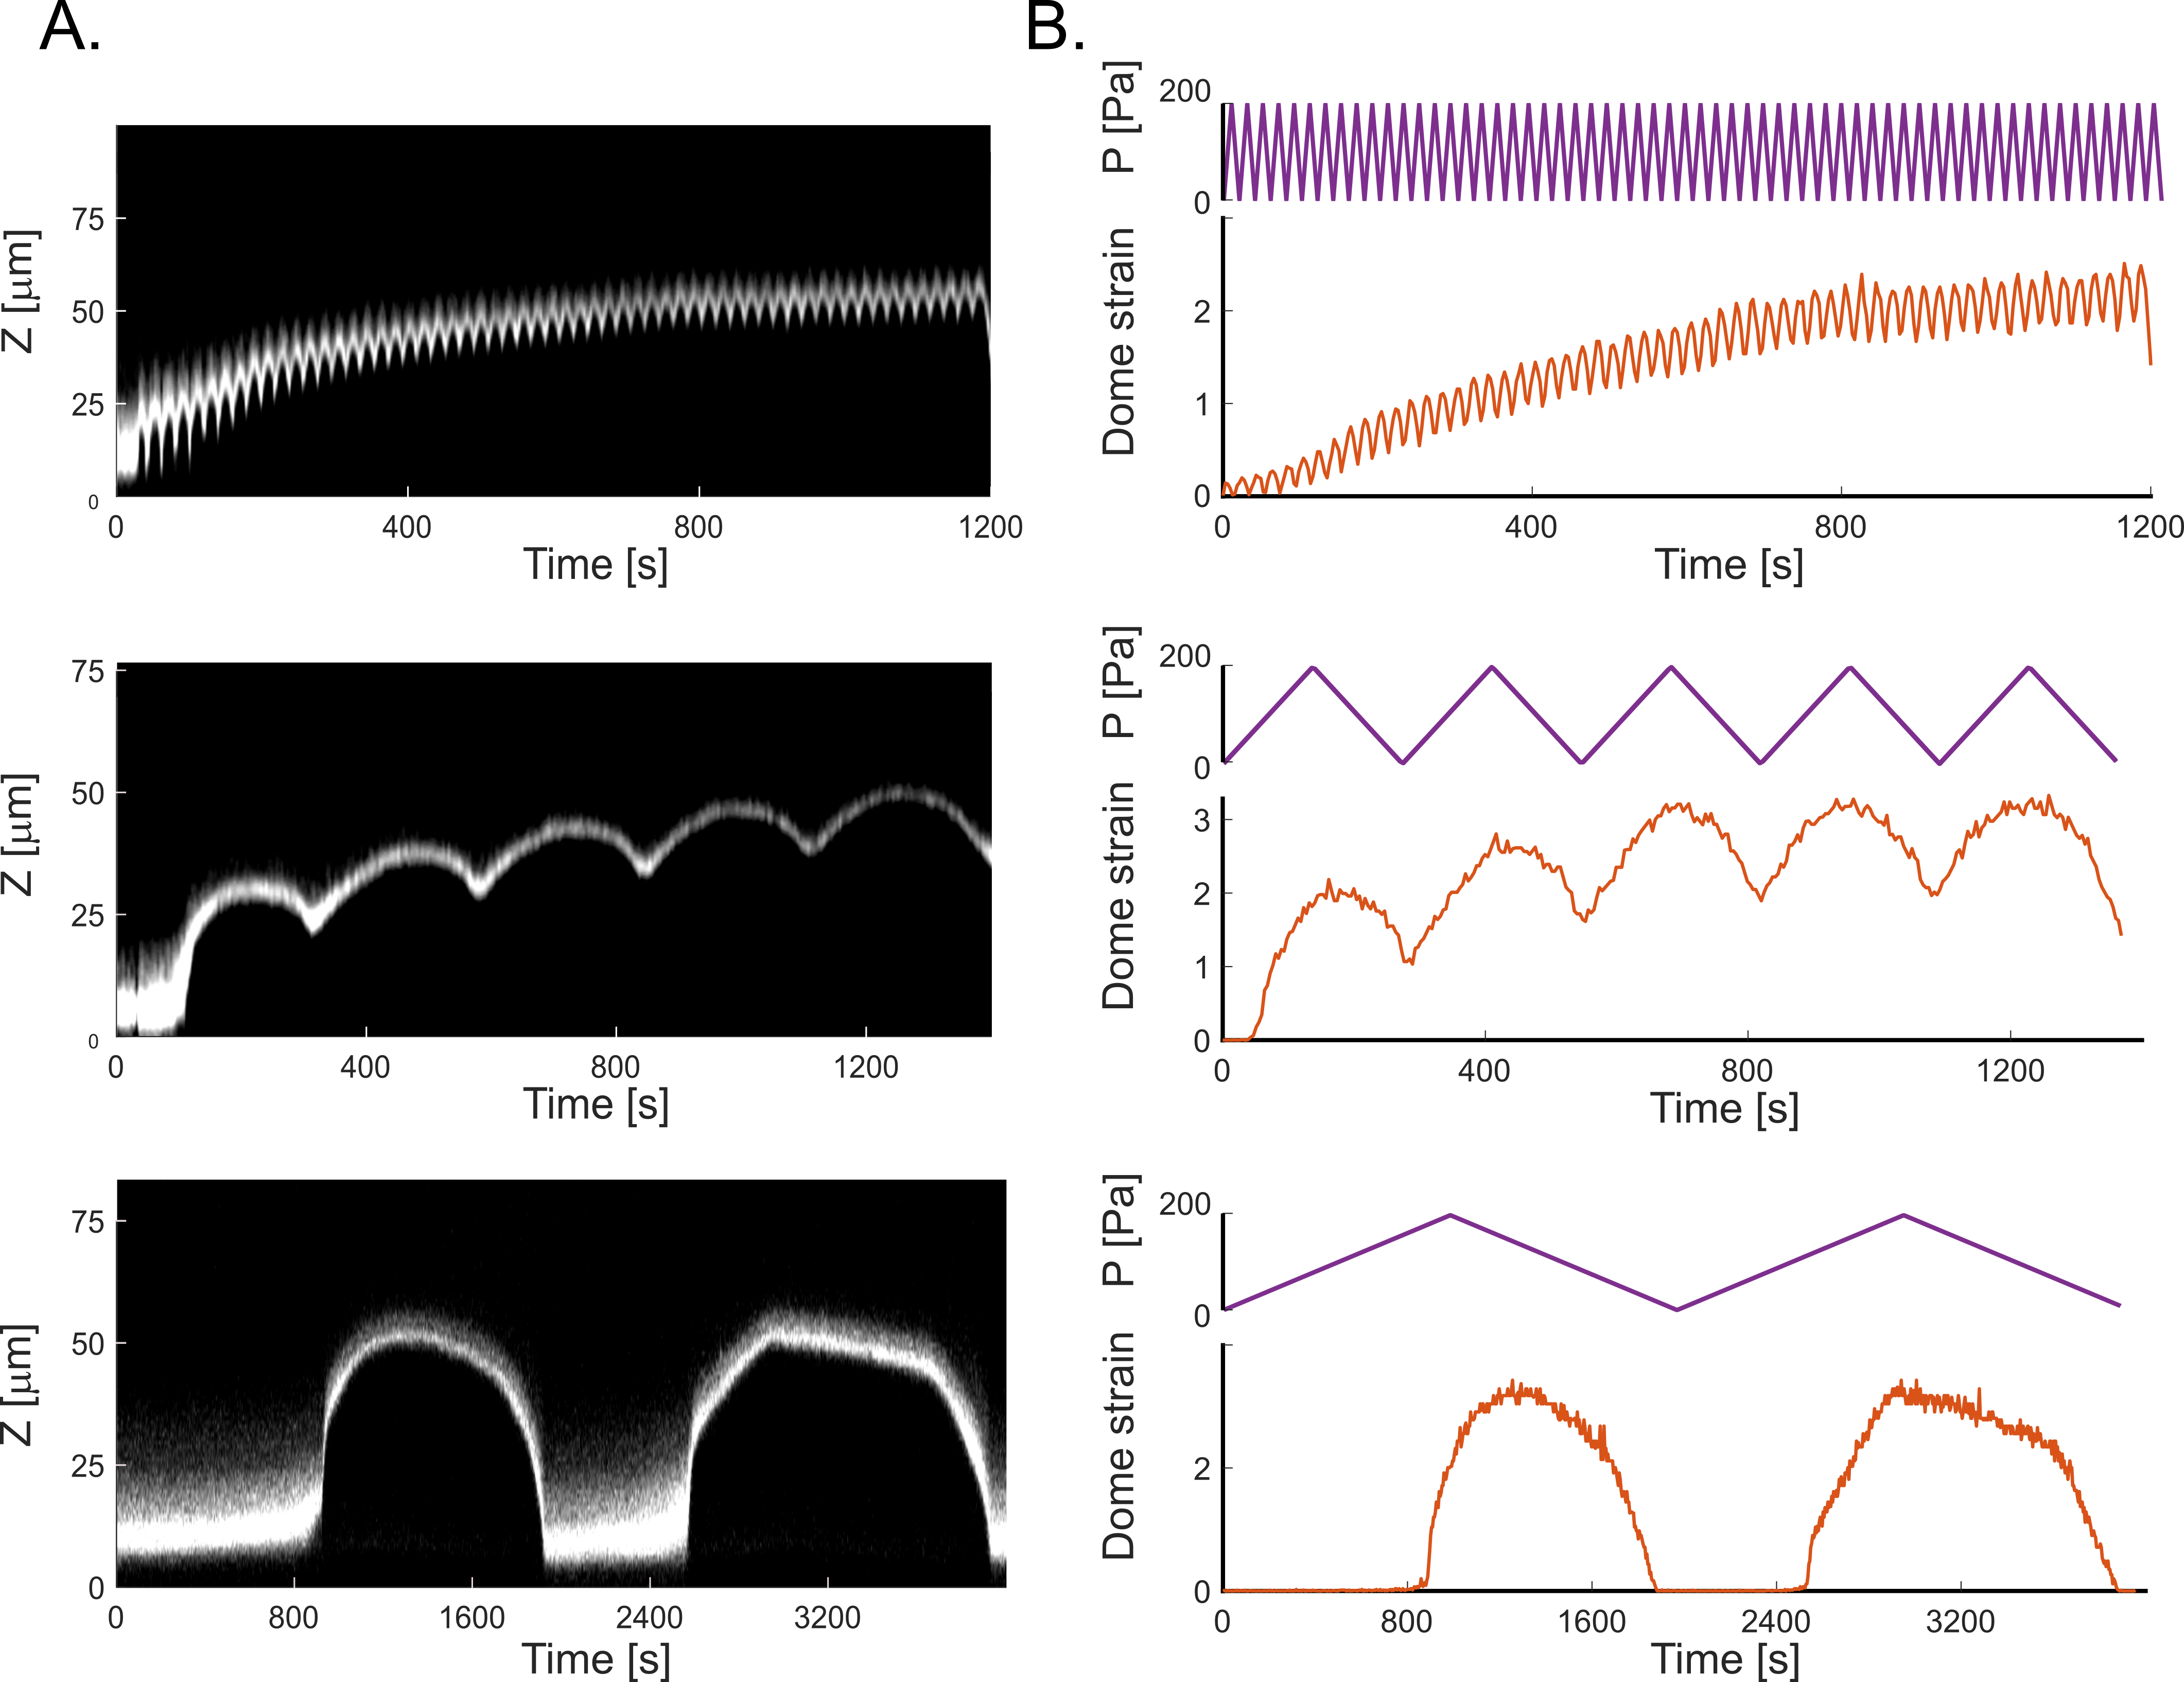
\includegraphics[width=\textwidth]{chap7_dynamic.png}
	\caption{\label{fig_7_6} \textbf{Dynamic response of Epithelia:} (A) The XZ plane images and kymographs of domes subjected to cyclic pressure between 0 to 200 Pa with rates of 20, 1.5, and 0.2 Pa/s The kymographs generated along the midsection of the domes indicated by yellow dotted lines. These indicate the evolution of height of the domes with respect to time. (B) The strain response of domes to cyclic pressure with different rates. Magenta represents pressure and red represents strain with respect to time. For A, B, n= 7 domes for 20 Pa/s, n = 8 for 1.5 Pa/s, and n = 7 for 0.2 Pa/s. 
	}
\end{figure}

In the case of the fastest cycles, we observed that the domes progressively stretched more as the cycles progressed until they reached a steady state oscillation. We conducted the experiment for $1200 s$ (60 cycles) and noticed that the domes accumulated strain progressively. While loading, they stretched, and while unloading, they unstretched but did not return to zero strain after the first few cycles. In the last few cycles, we observed that the dome oscillated between two states of strains.

A similar response was observed for the moderate cycles, where the domes were stretched for five cycles of $266 s$ each. The strain accumulated in the first cycle itself, with strains reaching higher values than those observed in the fast case. Additionally, after a few cycles, the dome appeared to have reached a steady state.

For the slowest cycles of $2000 s$, we faced difficulty in forming domes at lower pressures. As previously mentioned, the domes did not detach until they reached a critical pressure of $100-150 Pa$, after which they rapidly inflated to high strains of $200-300\%$. However, it was evident that the strains did not accumulate, and there was no difference in the maximum strains achieved in both cycles, indicating that the steady state was reached immediately at this timescale.

\hypertarget{active-gel-tissue-model}{%
	\section{Active gel tissue model}\label{active-gel-tissue-model}}

\begin{figure} [h!]
	\centering
	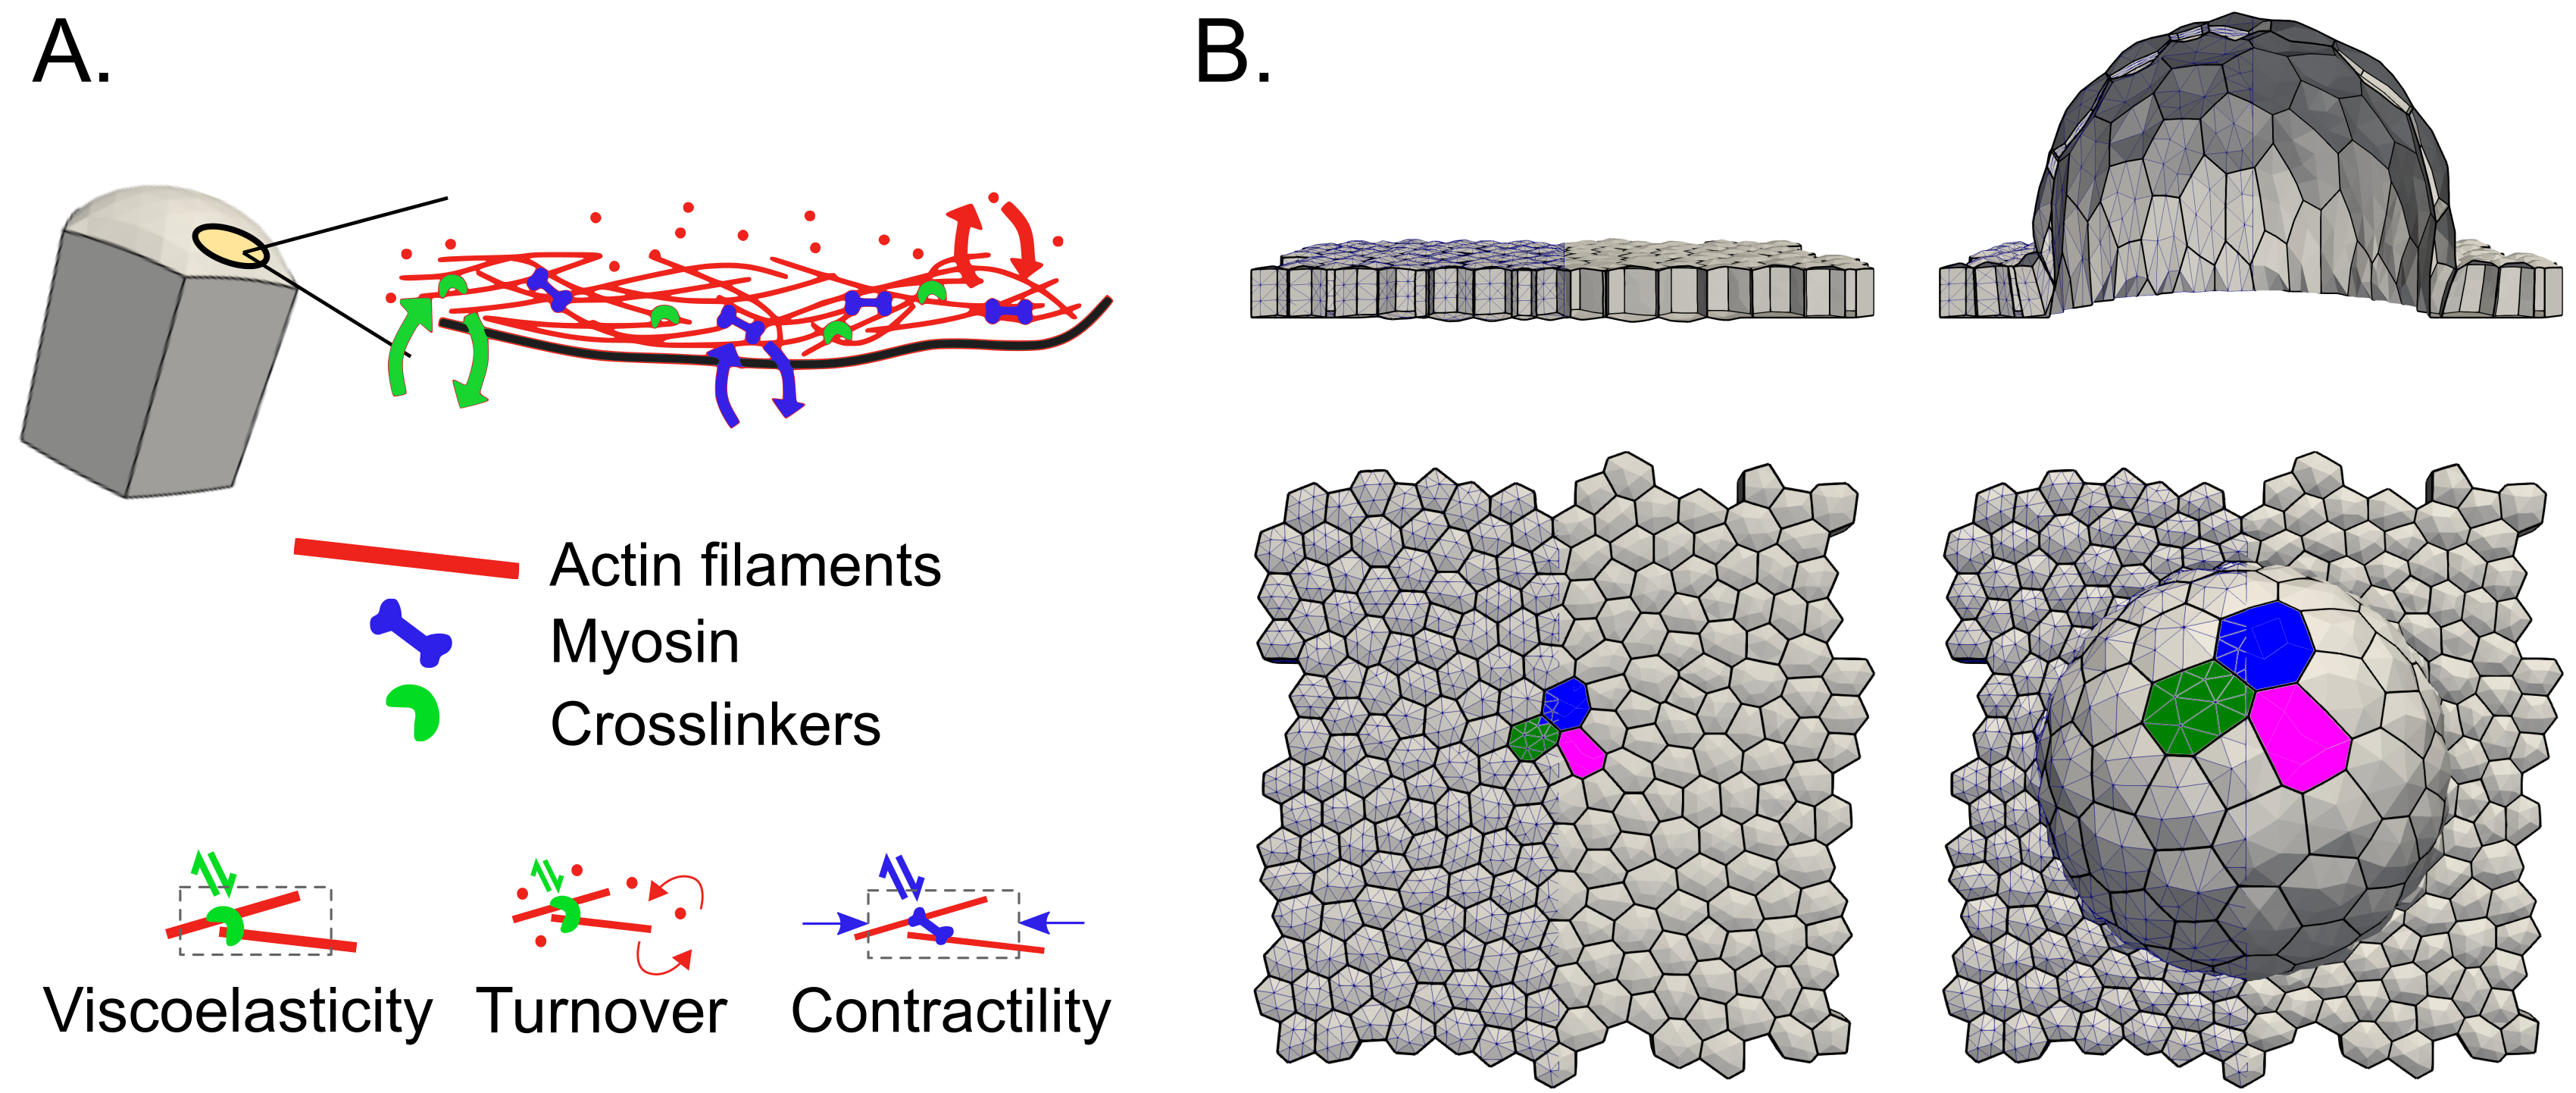
\includegraphics[width=\textwidth]{chap7_digitaldome.png}
	\caption{\label{fig_7_2} \textbf{Active gel tissue model}: (A) The cell is modeled as an active gel of cortex, which mainly comprises three aspects: viscoelasticity of the network, turnover dynamics, and active contractility. (B) These cells can be assembled into a tissue that can be used to perform in-silico experiments. An example of this is the digital dome being inflated, highlighting individual cells increasing their area.}
\end{figure}

In addition, to complement our experimental findings, we collaborated with Adam Ouzeri to develop a computational framework. Our understanding of epithelial mechanics suggests that the viscoelasticity of the actin cortex plays a crucial role in sustaining deformations at the timescale of seconds to minutes \cite{kelkar2020,clement2017,khalilgharibi2019}. Adam Ouzeri developed a theoretical framework that bridges active gel models of the actomyosin cortex and 3D vertex models at tissue scales  \cite{ouzeri2023}. In this model, each cell is represented by an active gel surface that accounts for the physical aspects of the cortex, and a tissue is assembled from a collection of these active gel surfaces (see fig \ref{fig_7_2}). The dynamics of the system are formulated through a balance of different potentials that represent different active internal or external forces and dissipation.

The framework accounts for the molecular dynamics of the actin filament network, myosin, and crosslinker proteins through four main components:

\begin{enumerate}
	\item \textbf{Cortical thickness:} The cell cortex is modeled as a hyperelastic membrane with cortical thickness ($\rho_R$). The deformation kinematics of this model is defined by mapping a cortical patch from a reference configuration ($\Gamma_0$) to a deformed configuration ($\Gamma$) with metric tensor \footnote{Metric  tensor, a mathematical object used in differential geometry, can be used to measure distances, angles, and volumes in curved spaces. Here, its measuring the cortical surface.} ($\mathbf{G_0}$) to ($\mathbf{g}$), respectively. To capture remodeling of cortex, the reference configuration has to be dynamic as well. Thus, there is a second reference configuration with a dynamic metric tensor ($\mathbf{G}$). The cortical thickness in the reference configuration changes with the mapping change represented by the Jacobian ($J_R$). This is expressed as 
	$$\rho_R(\mathbf{\xi}, t) = \rho(x,t)J_R(\mathbf{\xi},t).$$
	\item \textbf{Network elasticity:} This potential accounts for the free energy of the system undergoing deformation. The potential is dependent on the difference between in-plane strain ($\mathbf{C}$) and the metric ($\mathbf{G}$) written in the format of a hyperelastic potential ($W$). Using a Neo-Hookean elastic potential, $W$ depends on two Lamé parameters, ($\lambda$) and ($\mu$). This potential is expressed as $$\mathcal{F} = \int_{\Gamma_R} \rho_R \ W(\mathbf{C,G})dS_R.$$
	\item \textbf{Dissipation:} The actomyosin network remodels under tension, and the released elastic energy can be accounted for with a dissipation potential. The potential depends on a coefficient ($\eta$) equivalent to bulk viscosity, cortical thickness, and the rate of metric tensor given by ($\dot{\mathbf{G}}$). This potential is expressed as $$\mathcal{D} = \int_{\Gamma_R} \frac{\eta}{2}\ \rho_R \ \mathbf{\dot{G}}:\mathbf{\dot{G}} \ dS_R.$$
	\item \textbf{Active contractility:} The model is an active gel, and the active part is included through an active power potential that adds energy to the system. The potential is dependent on the cortical tension and the rate of deformation tensor. The cortical tension is an active tension component of the network that is proportional to cortical thickness. This potential is expressed as $\gamma(\rho) = \rho \xi$ and $$\mathcal{P} = \int_{\Gamma} \gamma : \mathbf{d} \ dS.$$
	
\end{enumerate}

Additionally, we account for turnover dynamics in the cortex through a mass balance law. Here, we assume that there is a steady-state cortical thickness, and the network is constantly polymerizing and depolymerizing with cytosolic components. This is expressed as $$\dot{\rho} + \rho \ tr(\mathbf{d}) = k_p\ C - k_d\ \rho.$$

The proposed governing equations are obtained by minimizing the Rayleighian, which is given as:

$$ \mathcal{R} = \frac{dF}{dt} - D + P + P_e .$$

Here, $P_e$ is an additional potential that accounts for external forces and tractions. The model assumes that the volume of the cell is conserved during deformation, and a mechanical barrier is introduced to prevent excessive strains beyond a threshold. This barrier is implemented by adding re-stiffening at large strains, which is necessary for physiological reasons, such as activation of intermediate filaments, cell crowding, or compression of the nucleus.

The model exhibits three timescales: turnover time ($t_{to} = 1/k_d$), viscoelastic time ($t_{ve} = \eta/\lambda$), and viscoactive time ($t_{va} = \eta/\xi$). At shorter timescales, the system behaves like an active hyperelastic material, while at longer timescales, it behaves like an active viscoelastic material.

Adam Ouzeri was able to implement this model in our system by creating a digital twin of the monolayer consisting of cell membranes. Non-adhesive regions were also included, which could be inflated into domes under pressure, similar to the experimental setup. Here after, we will refer to them as "digital domes" (see fig. \ref{fig_7_2}).

\hypertarget{active-viscoelasticity-of-the-epithelia}{%
	\section{Active viscoelasticity of the
		epithelia}\label{active-viscoelasticity-of-the-epithelia}}
	
\begin{figure}
	\centering
	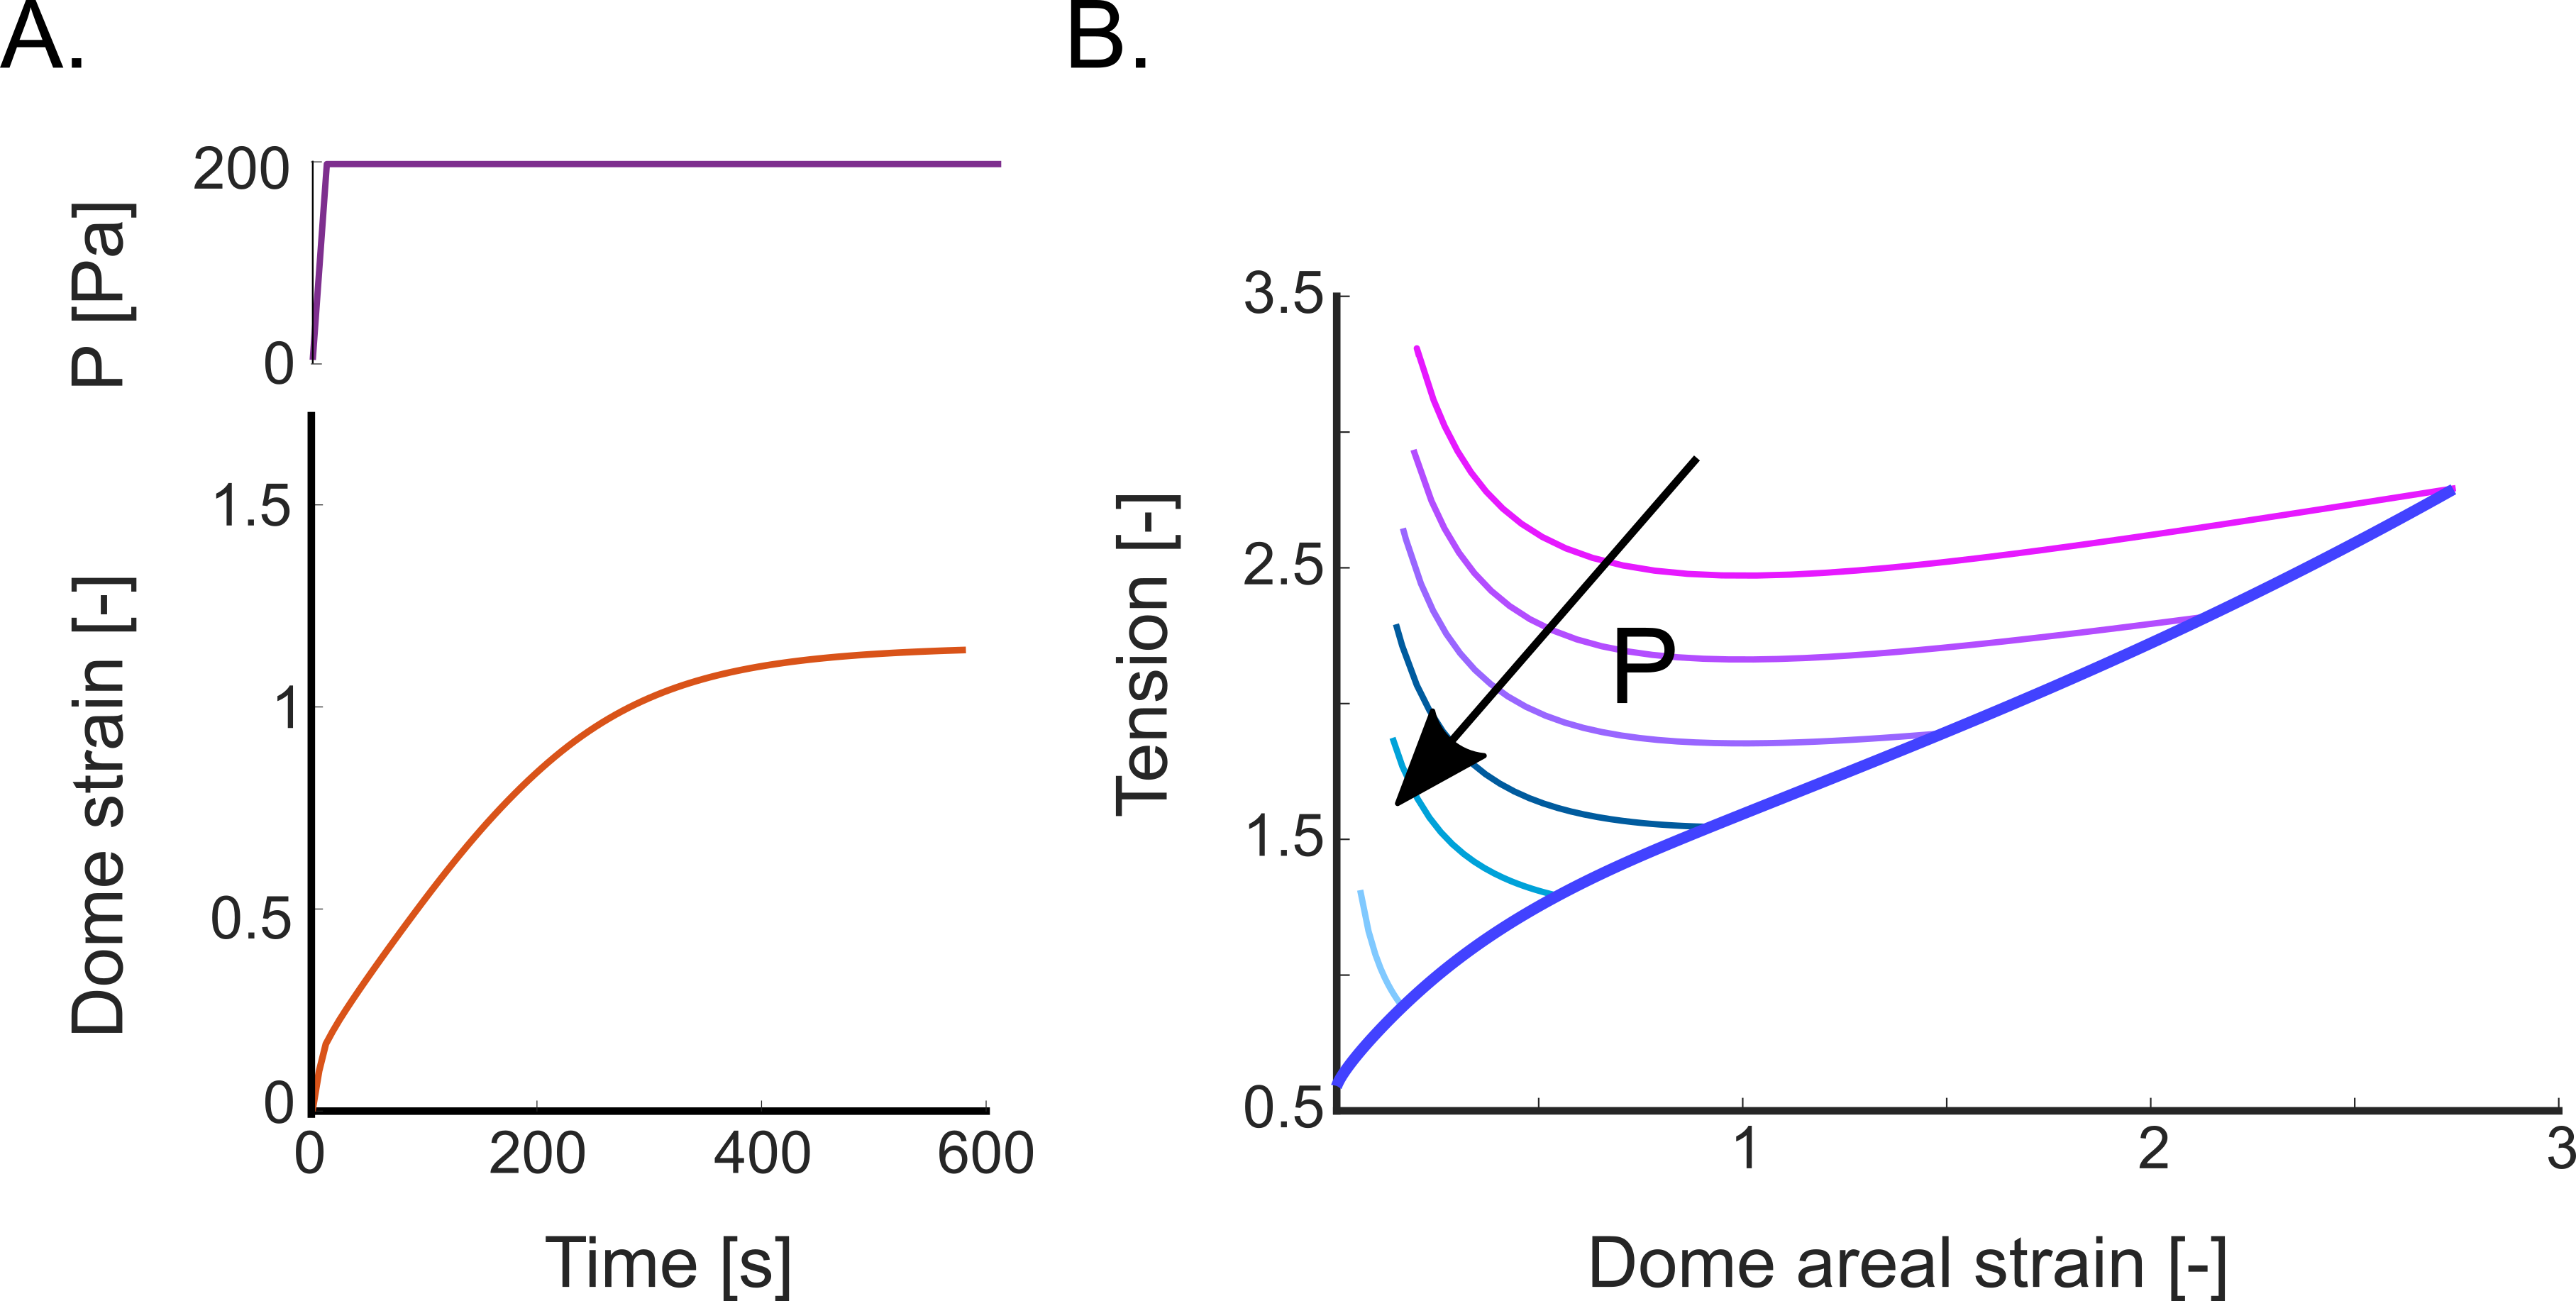
\includegraphics[width=\textwidth]{chap7_constitutivelawtwin.png}
	\caption{\label{fig_7_7} \textbf{Material response of the digital domes}: (A)  When subjected to constant pressure, as in experiments, the digital dome inflated and reached a steady state. (B)  These simulations also produced isobarics for different pressures, all leading to a steady state. Furthermore, subjecting it to a quasi-static increase in pressure produced a constitutive law (Navy blue curve) that can be mapped onto the locus of steady-state points.}
\end{figure}


By conducting simulations that mirror the experimental conditions, we were able to gain insights into the mechanics of the system. Specifically, we found that when digital domes were inflated with constant pressure, they reached a steady state while experiencing a reduction in cortical thickness as the cells stretched. Once the tissue tension was balanced by the applied pressure, the strain reached a stable point (see fig \ref{fig_7_7} A).

To evaluate the constitutive relation provided by the model, we inflated the digital dome with different pressures to obtain isobaric curves and steady state points. We also inflated a digital dome quasi-statically, though this is not feasible in experiments, to assess the model's robustness. We discovered that the constitutive relation obtained quasi-statically was consistent with the steady state locus in the isobarics  (see fig \ref{fig_7_7} B). The constitutive curve exhibits similar characteristics to experiments, including clear re-stiffening at large strains, which we attribute to a barrier mechanism.

We interpreted these findings in light of the concept of resting area, which refers to the area of a cell in a monolayer that is in a steady state. When the tissue is perturbed from this state, the actual area changes faster than the resting area due to the viscoelastic behavior of the tissue. The cell can dissipate elastic stresses at viscoelastic timescales through remodeling, eventually reaching a steady state. This effect of timescales is particularly evident in cyclic stretching experiments. When the cells are probed faster than viscoelastic timescales, they accumulate strains due to an inability to dissipate the elastic stress. In contrast, when stretching is slower, elastic stresses are dissipated with increasing area.

We observed that, for the slowest condition, the resting area in the digital dome almost overlapped with the actual area. This is because the pressure is changing very slowly at a rate of 0.2 Pa/s, allowing the cells sufficient time to remodel and dissipate elastic stresses. Viscoelastic and turnover timescales in simulations are around 10-30s, which means that over a period of 2000s, the dome stretches considerably and returns to original flat state.

However, when pressure is applied rapidly in cycles of 20 seconds, strains accumulate due to insufficient time for cells to dissipate stored elastic energy. Our simulations show that the resting area marginally changes relative to the actual area. Notably, creep experiments, where tissue is stretched at constant tension, demonstrate strain accumulation at the visco-active timescale, where both contractility and viscosity play a role. 

Interestingly, our simulations indicate that due to active viscoelasticity, there would be a lag between the peak of pressure and the peak of strain. This lag is clearly reflected in the comparison of resting area and actual area, where the delay decreases with increasing pressure rates. The slowest pressure rate results in the least amount of delay, while the fastest pressure rate results in the most delay. although we can only experimentally observe this at moderate rates. The experimental data from faster cycles is too noisy to observe the lag.

To sum up, the digital dome model explains the different behaviors of epithelial tissue depending on the rate at which pressure is applied. Slower rates allow for cell remodeling and dissipation of elastic stresses, while faster rates result in strain accumulation due to insufficient time for dissipation.

\begin{figure}
	\centering
	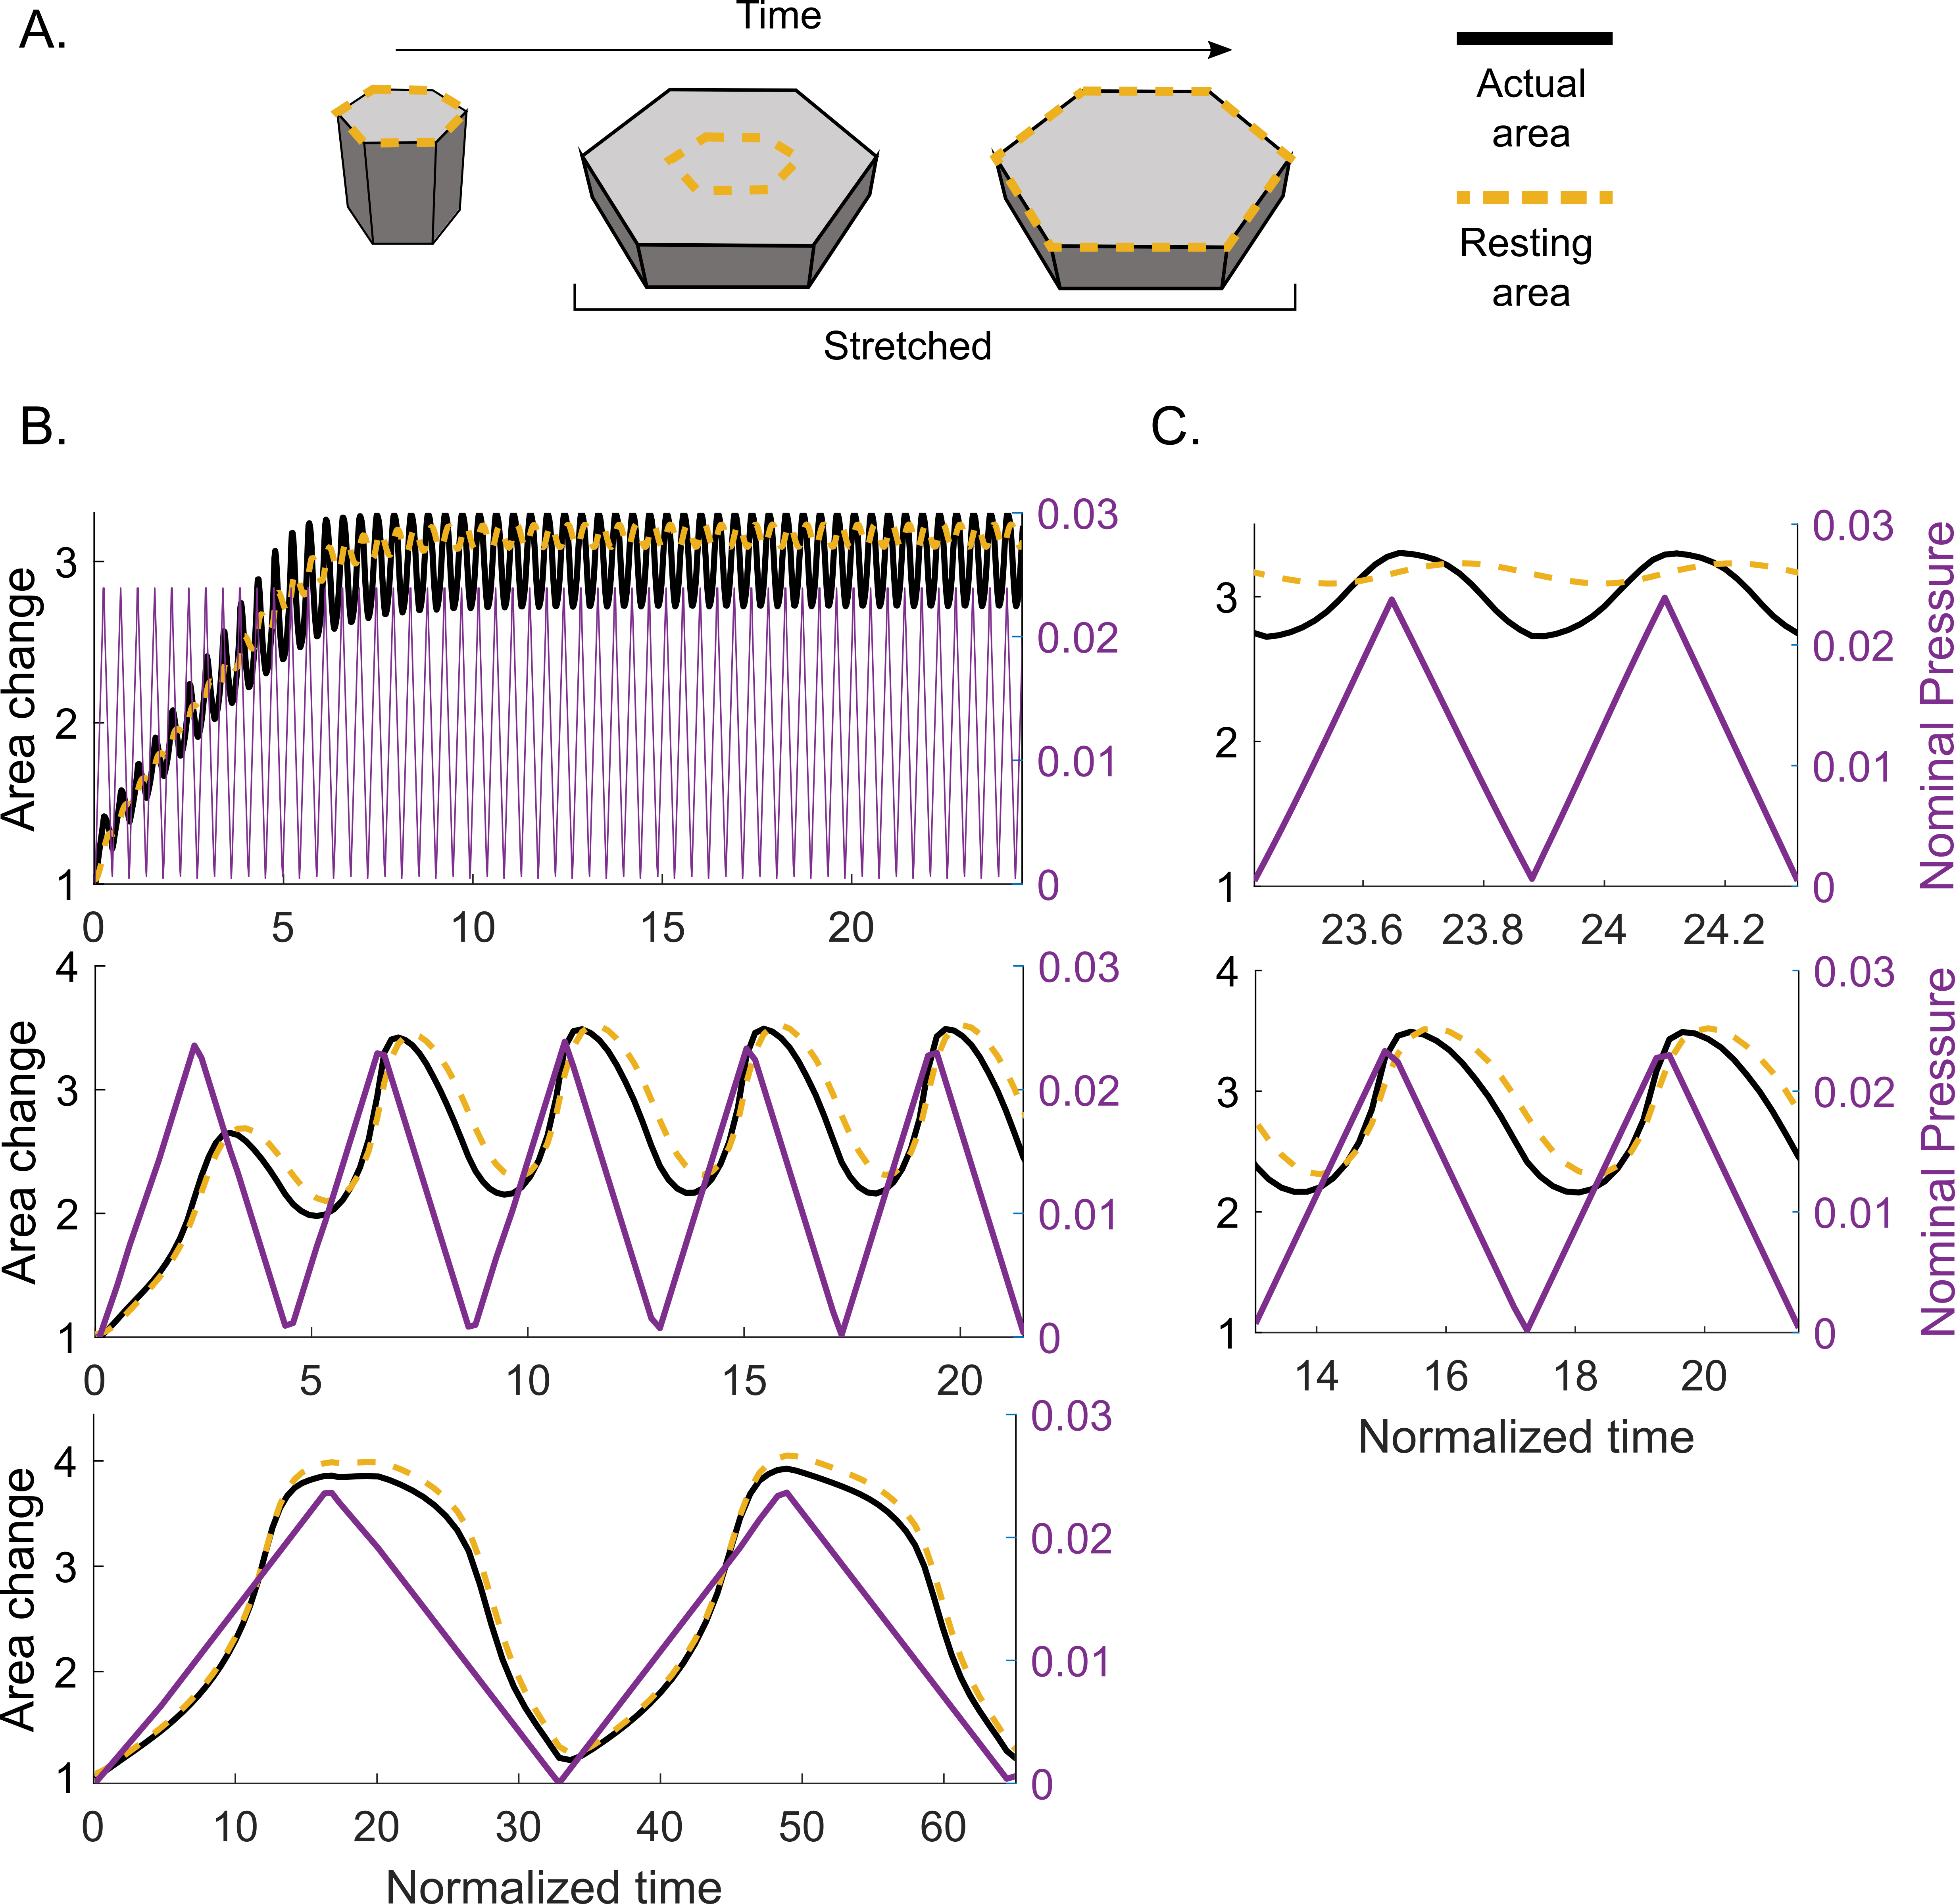
\includegraphics[width=\textwidth]{chap7_area.png}
	\caption{\label{fig_7_8} \textbf{Concept of resting area}: (A) Illustration of a resting and actual are of a cell in a monolayer during stretching. (B) Differences in results of resting and actual area when subjected to different rates of pressure. (C) Inset of the last two cycles.
	}
\end{figure}

\hypertarget{summary}{%
	\section{Summary and Discussion}\label{summary}}

In this study, we investigated the mechanics of epithelial tissue by applying pressure at varying rates. Initially, we applied a constant pressure of $200Pa$, which led to the dynamic inflation of domes and eventually reached a steady-state in strain. Due to the spherical geometry of the tissue, we observed a non-monotonous tension-strain curve in response to the constant pressure. However, we found that the true tension-strain curve exhibited increasing tension with respect to strains at lower values, but at higher strains, the tension appeared to be independent of the strains.

Furthermore, our results showed that the domes accumulated strain through the cycles when probed with fast-changing pressure and reached a steady-state in later cycles. However, when stretched slowly, the domes stretched to high strains without accumulating strain.

To understand the behavior of epithelial tissue, we developed an active viscoelastic fluid model, which allowed us to probe the time-dependent response of the tissue to pressure. Our experimental and computational framework show that the response of the domes to cyclic pressure is dependent on active viscoelasticity.

The tissue stretches to balance the tissue tension with externally applied pressure timescale and reaches a steady-state strain by actively remodeling the cortex. Our digital dome studies indicated that different timescales play a role together in producing the tissue's response to pressure. These timescales are the reflection of  interplay between cortical turnover, crosslinkers, and network reorganization which allows for large deformations and rapid shape changes.

Our results can be interpreted using a multidimensional Maxwell model, which is a model that describes viscoelasticity. The classical Maxwell model consists of a spring and a dashpot, which represent the elastic and viscous elements, respectively. In our case, we can imagine a similar model with two branches: one branch includes a spring and a dashpot to represent the passive viscoelasticity, and a second branch includes an active spring to represent the active component (see fig \ref{fig_7_9}). The active spring is always present, but if the stretching is done slowly, the dashpot would be driving the dominant mechanical response. Conversely, if the stretching is done rapidly, the elastic spring deformation would dominate. By separating the passive and active components, we can better understand how each contributes to the overall viscoelastic behavior and associated timescales.

\begin{figure}
	\centering
	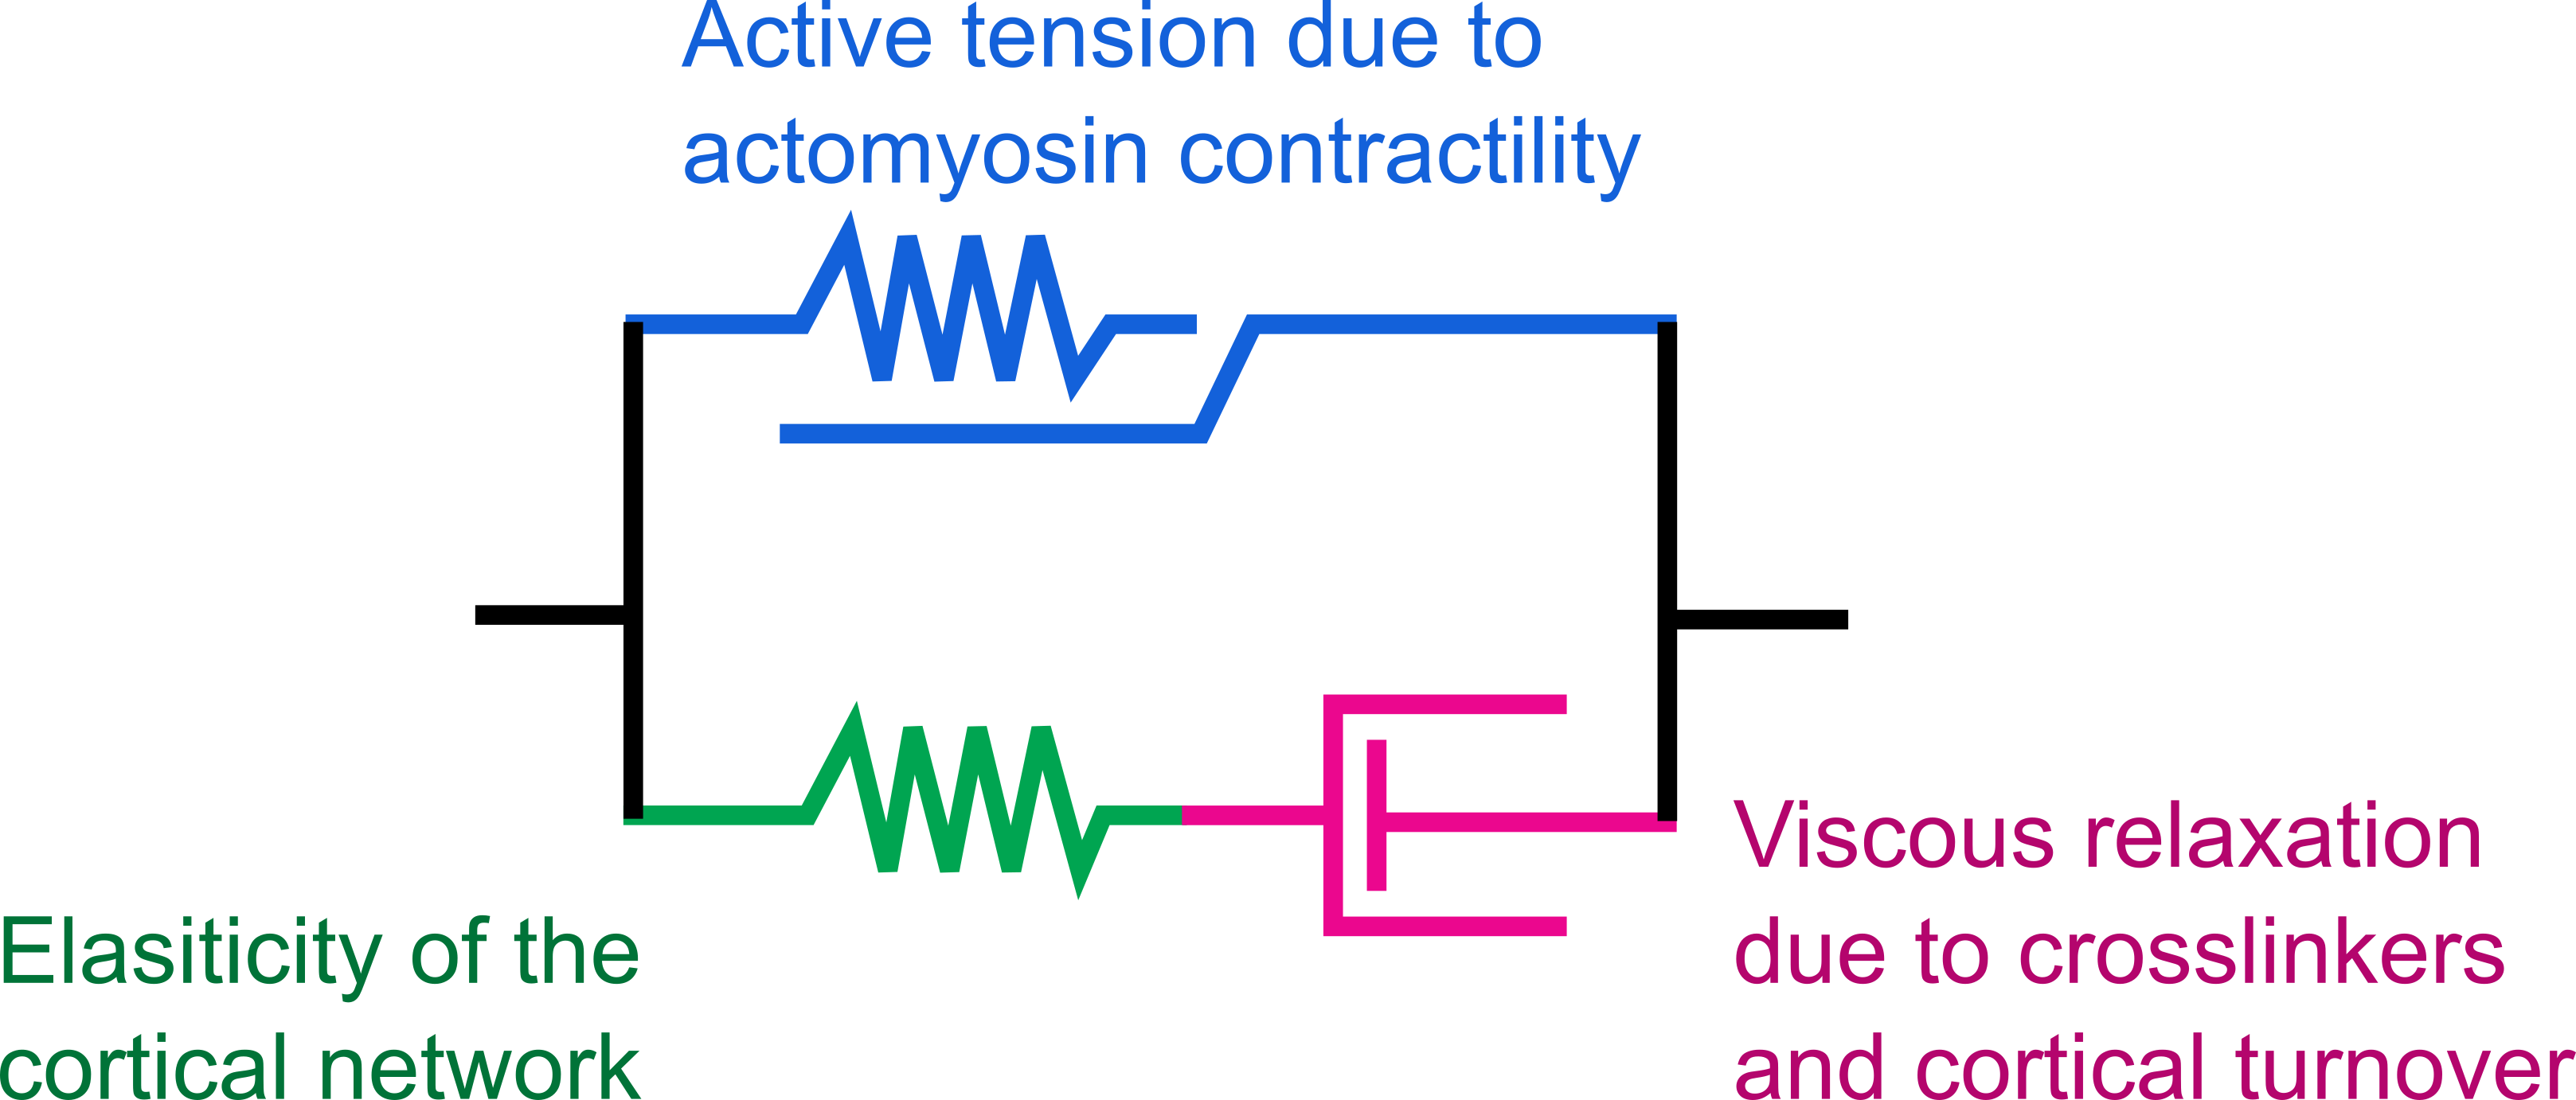
\includegraphics[width=0.75\textwidth]{chap7_maxwell.png}
	\caption{\label{fig_7_9} \textbf{Representational viscoelasticity model}: The model can be understood using a spring and dashpot analogy with two branches: The first branch is an active spring representing the contractile forces applied by the actomyosin cortex. The second branch has two components, one for the elasticity of the network and the second for the viscous relaxation that occurs due to turnover of the network.
	}
\end{figure}

Previous research has approached the system in a similar manner, where epithelial tissue was modeled using viscoelastic models of springs and dashpots. One particularly interesting model was developed by Khalilgharibi et. al., which characterizes the response of a suspended monolayer to stretch and demonstrates that the dynamics are similar to that of a single cell, due to the role of the actomyosin cortex \cite{khalilgharibi2019}. They used a model with two springs in parallel, one of which can change its length dynamically. This explains the relaxation of the monolayer, where the active contractility of the cortex changes the resting length of the active spring in the model, which closely relates to our "resting area" concept.

Another study found that viscoelastic dissipation could explain the shortening or elongation of cell junctions in drosophila embryos \cite{clement2017}. They demonstrated that the dissipation occurs at the minute timescale, at the same timescale as myosin pulses. It is also interesting that they found actin turnover plays a key role in this dissipation.

Applying tensions and strains to suspended cells in vitro is a challenging task, and it is important to note that adherent monolayers may exhibit different behaviors from suspended cells \cite{harris2012}. The tissue matrix provides additional stiffness and can alter the cytoskeletal structure of cells, which further complicates the understanding of cell mechanics \cite{humphrey2014, kechagia2019}. In this thesis, we focus specifically on the actin cortex and short timescales (minutes).

The timescale of actin remodeling is on the order of tens of seconds, and we did not observe any cellular rearrangement or division at this timescale in our system (with rare exceptions). Long-term experiments were not performed due to suspected involvement of other cytoskeletal components, such as intermediate filaments. In a study by Latorre et al., activation of intermediate filaments was observed in extremely stretched cells ($>300\%$), which caused re-stiffening and prevented the cells from stretching too much \cite{latorre2018}. This motivated the strain limiting mechanism imposed in our model. However, in our experiments, we did not observe any indication of superelasticity, as all cells were super-stretched at the same time. This might be due to the relatively shorter timescales in our experiments compared to long term quasi-static deformation of spontaneous domes.

\textbf{About strain stiffning and results of \cite{duque2023}. About racheting of contractile force \cite{clement2017, mason2011} and strain accumulation or creep}

In the next chapter, we will endeavor to apply our understanding of viscoelasticity to generate radical transformation of domes into various structures.